\documentclass[a4paper,12pt]{book}
\usepackage[utf8]{inputenc}
\usepackage[T1]{fontenc}
\usepackage[brazilian]{babel}
\usepackage{graphicx}
\usepackage{hyperref}
\usepackage{amsfonts}
\usepackage{amsmath}
\usepackage{dsfont}
\usepackage{algorithm}
\usepackage{algorithmic}
\usepackage{breqn}
\usepackage{graphicx}
\usepackage{subcaption}
\usepackage{natbib}
\usepackage{caption}
\usepackage{epigraph}
% usado pra pseudo-codigo
\renewcommand{\algorithmicrequire}{\textbf{Input:}}
\renewcommand{\algorithmicensure}{\textbf{Output:}}

\graphicspath{{./imagens/}}

% operacoes do SVM
\DeclareMathOperator*{\argmax}{argmax}  
\DeclareMathOperator*{\argmin}{argmin}  

\hypersetup{
	colorlinks=true,
	linkcolor=blue,
	urlcolor=red,
	linktoc=all
}

\newenvironment{dedication}
  {\clearpage           % we want a new page
   \thispagestyle{empty}% no header and footer
   \vspace*{\fill}% some space at the top 
   \itshape             % the text is in italics
   \raggedleft          % flush to the right margin
  }
  {\par % end the paragraph
   \clearpage           % finish off the page
  }

\usepackage{etoolbox}
    \makeatletter
    \newlength\epitextskip
    \pretocmd{\@epitext}{\em}{}{}
    \apptocmd{\@epitext}{\em}{}{}
    \patchcmd{\epigraph}{\@epitext{#1}\\}{\@epitext{#1}\\[\epitextskip]}{}{}
    \makeatother

\begin{document}


\frontmatter
\begin{titlepage}
	\centering
	{\scshape\LARGE Instituto de Matemática e Estatística \par}
	\vspace{1cm}
	{\scshape\Large Trabalho de Formatura Supervisionado\par}
	\vspace{1.5cm}
	{\huge\bfseries Análise de Sentimentos Aplicada à Política\par}
	\vspace{2cm}
	{\Large\itshape Lucas Romão Silva\par}
	\vfill
	Orientado por\par
	Prof. Dr. Roberto Hirata Jr. 

	\vfill

% Bottom of the page
	{\large \today\par}
\end{titlepage}

\begin{dedication}
À minha mãe, Claudete Romão Silva
\end{dedication}
\chapter*{Agradecimentos}

Ao meu orientador, Roberto Hirata Jr. pois sem seu auxílio e orientação este trabalho não
seria possível.

À minha família que sempre me apoiou ao longo desta graduação em especial à minha irmã Sarah
que foi um grande apoio para mim e com certeza sem ela não teria conseguido ir até o fim.

Aos meus amigos que me apoiaram e me ajudaram ao longo de toda a jornada. Em especial
à família do paninho, Antonio Abello, Alice Dias, Caroline Gonçalves, Cesar Cano, Cristiane Augusta
Gabriel Nascimento e João Luciano por ficarem ao meu lado e me ajudar em diversos momentos importantes ao longo deste ano, sejam eles diretamente ligados à academia ou não.
\chapter*{Resumo}

Com a grande expansão da internet, o uso das redes sociais tem se
tornado cada vez mais ativo e, com o passar do tempo, tornou-se um
lugar onde os usuários relatam não só informações acerca do cotidiano,
mas também para opinar sobre temas como política, esportes, etc. O uso
 das redes sociais também causa maior mobilização dos usuários no
cenário político através de petições online ou organização de
manifestações.

Este trabalho tem como objetivo explorar a rede de usuários do Twitter
para analisar os sentimentos dos seus usuários acerca do cenário
político brasileiro atual utilizando técnicas de processamento de
linguagem natural em conjunto de técnicas de aprendizado de máquina.

Para isso coletou-se tuítes sobre grandes decisões atuais como: (1) a
Reforma da Previdência (PEC287); (2) a proposta de Lei da
Terceirização; (3) a proposta de emenda constitucional sobre o Teto
dos Gastos Públicos (PEC55); além de tuítes sobre políticos em grande
visibilidade no cenário político atual.

Os tuítes coletados foram classificados manualmente através de uma
ferramenta desenvolvida neste TCC (um site na Internet) onde era
possível realizar a tarefa de classificação de forma menos árdua e
permitir a ajuda de outras pessoas.

A preparação dos dados foi feita através de técnicas de processamento
de linguagem natural para extrair informações subjetivas dos tuítes e
classificou-se as opiniões associadas a eles utilizando técnicas de
aprendizado de máquina.

Induzidos os classificadores, analisou-se métricas de desempenho de
cada um como Acurácia, Precisão e Revocação para diferentes abordagens
de extrair as informações subjetivas do texto.
Como resultado, obteve-se uma acurácia média de 71\%.



\vspace*{\fill}
    \epigraph{A utopia está lá no horizonte. Me aproximo dois passos, ela se afasta dois passos. Caminho dez passos e o horizonte corre dez passos. Por mais que eu caminhe, jamais alcançarei. Para que serve a utopia? Serve para isso: para que eu não deixe de caminhar.}{Fernando Birri}


\tableofcontents

\mainmatter
\chapter{Introdução}

A expansão da internet impulsionou o uso cada vez maior das redes sociais por cada vez mais
usuários. Segundo estudo realizado pelo portal Statisa\cite{statisa}, em 2017 existe
2,46 bilhões de usuários nas redes sociais do mundo todo.

As redes sociais tornaram-se um local para a manifestação de opinião dos usuários acerca de
diversos assuntos. Dentre as principais redes sociais, o twitter possui na comunidade brasileira
a maior quantidade de usuários fora dos Estados Unidos com 27,7 milhões de usuários.
Estudos recentes do Twitter Brasil mostram que o país foi o terceiro em maior crescimento em número
de usuários no ano de 2016, avançando em 18\% o número de usuários que utilizam a rede social ao
menos uma vez por mês em relação ao mesmo estudo realizado em 2015.\cite{twitterFolha}

Motivado pela popularidade do Twitter em uma parcela da população brasileira, aliada à facilidade
de obter-se dados postados na rede social decidiu-se analisar as opiniões dos usuários do Twitter
acerca do cenário político brasileiro atual construindo classificadores de tuítes onde cada
tuíte era classificado como opinião positiva, negativa ou neutra e estudar como
cada classificador e forma de representação dos dados contribui para a construção de um bom
classificador. 

Para isso, coletou-se tuítes de julho de 2016 a julho de 2017 sobre as reformas da previdência, lei
da terceirização, a proposta de emenda constitucional do teto dos gastos e sobre políticos
com notoriedade no cenário brasileiro atual como os ex-presidentes Luis Inácio Lula da Silva,
Dilma Rouseff e o senador Aécio Neves.

Além disto este trabalho se propôs a construir uma ferramenta (na forma de um site) que permite
facilitar a tarefa da classificação manual de dados textuais e a colaboração de mais usuários.

Este trabalho é organizado da seguinte forma: o capítulo 2 tratará da revisão dos estudos mais
recentes na literatura quanto ao uso do Twitter em tarefas de análise de sentimentos voltada à
política. O capítulo 3 trata da fundamentação teórica não só acerca dos métodos de aprendizado de
máquina, mas também técnicas de representação dos tuítes e um detalhamento do funcionamento e motivação
da criação da ferramenta para a classificação manual dos dados. No capítulo 4 são discutidos os resultados
dos algoritmos desenvolvidos e é realizada uma comparação destes com as implementações já existentes
na biblioteca \texttt{scikit} do Python. Por último no capítulo 5 são discutidos melhorias dos resultados
atuais e perspectivas futuras acerca deste trabalho.
\chapter{Materiais e Métodos}

\section{Considerações}
\label{sec:considerations}

Ao longo deste capítulo, se usará n para se referir à quantidade de elementos
fornecidas ao nosso modelo, cada entrada é i é um vetor $x_i \in \mathbb{R}^m$.
Para cada i associaremos duas variáveis $t_i$ e $y_i$ que se referem ao valor
esperado e ao valor obtido através do treinamento, respectivamente. 

\section{Contextualização}
\label{sec:methods}

Os problemas tratados por \textit{Machine Learning} classificam-se de forma
geral em três tipos:

\begin{itemize}
	\item Aprendizado supervisionado: nesse caso tem-se os elementos de entrada e
	para cada um desses elementos, tem-se associado um rótulo $t_i$. Nesse caso o modelo
	deve ser treinado com base nos elementos dados para que se possa prever o rótulo %não consegui pensar numa tradução boa pra label%
	de uma nova entrada;
	\item Aprendizado não-supervisionado: nesse caso tem-se apenas os elementos de entrada. 
	O objetivo deste tipo de problema é tentar modelar uma distribuição ou estrutura comum
	entre os dados para que se possa entendê-los melhor;
	\item Aprendizado semi-supervisionado: nesse último caso alguns elementos possuem um rótulo
	associado. Problemas desse tipo aplicam técnicas gtanto de aprendizado supervisionado como
	de não-supervisionado.
\end{itemize}

Neste trabalho será tratado um problema de aprendizado supervisionado que é o da classificação.

Na classificação temos k classes e cada elemento i da entrada é associado a uma classe $t_i = \{1..k\}$.
O objetivo do problema da classificação é dado entrada $X = (x_1, x_2, \ldots, x_n)$ 
e $t = (t_1, \ldots, t_n)$ treinar um modelo capaz de prever classes para um x qualquer.

Há diversos algoritmos na literatura que se propõem a resolver o problema da classificação.
Bishop (2006)\cite{bishop2006} enuncia diversos dos algoritmos comumente utilizados para a
classificação, cada algoritmo possui seus prós e contras e utiliza diferentes abordagens.

Para este trabalho escolheu-se implementar os algoritmos \textit{Logistic Regression} e
\textit{Supor Vector Machines}, que será chamado simplesmente de SVM por facilidade.

Tanto para o \textit{Logistic Regression} quanto SVM será explicado a princípio o problema
será inicialmente abordado a partir da classificação binária e, a partir dela, será descrito
como estender para o problema com mais de duas classes, que será é o caso deste trabalho.

\section{Logistic Regression}
\label{sec:logreg} 

Para classificar um dado elemento x entre as possíveis classes $C_1$ e $C_2$, é utilizado
um discriminante linear da forma $y(x) = w^Tx + w_0$ sendo w o vetor de pesos associado.
A classe atribuída a um vetor x é baseado no sinal de $y(x)$, se $y(x) \ge 0$ ele é designado
à classe $C^1$, caso contrário é designado à classe $C^2$.

No caso da classificação binária, usamos que $t_n \in \{0, 1\}$

Nesse caso, diz-se que uma superfície de decisão é definida pelo hiperplano $y(x) = 0$ onde
sua posição é determinada pelo elemento $w_0$ que chamaremos de viés. Uma vez que tanto nosso
vetor de pesos w quanto nossos vetores x do conjunto de treino possuem m elementos, iremos criar
vetores novos $w' = (w_0, w), x' = (1, x)$.

O nosso modelo será construído de forma probabilística, uma vez que o objetivo será obter um vetor
w de modo que possamos estimar as probabilidades condicionais $P(C^1 | x)$ e consequentemente
$P(C^2 | x) = 1 - P(C^1 | x)$, isto é, a probabilidade de um vetor x pertencer à uma determinada 
classe. 

Para utilizarmos nosso discriminante $y(x)$ para atribuir as probabilidades, utiliza-se a função
sigmóide definida por:

\begin{center}
	\begin{equation}
		\sigma(a) = \frac{1}{1 + exp(-a)}
	\end{equation}
\end{center}

Com $exp$ sendo a função exponencial. Aplicando ao nosso modelo obtêm-se a expressão:

\begin{center}
	\begin{equation}
		P(C^1 | x) = y(x) = \sigma(w^Tx)
	\end{equation}
\end{center}

Importante notar que apesar de utilizarmos o vetor x nas equações, é possível aplicarmos uma
transformação linear $\phi : \mathcal{R}^m \rightarrow \mathcal{R}^d$ à entrada x para obtermos
$\phi(x)$. O uso de transformação linear no nosso conjunto de entrada nos permite transformar o 
domínio para que se obtenha uma separação melhor entre as classes ou até mesmo fazer a redução
da dimensão do domínio.

Com essa equação em mãos, nosso objetivo é minimizar o erro na classificação dos dados. Tomamos
como erro o negativo do logaritmo da verosimilhança de nossa função que é dada por:

\begin{center}
	\begin{equation}
		E(w) = - \sum_{i = 1}^{n} p(t | w) = 
		- \sum_{i = 1}^{n} \{ t_nln(y_n) + (1 - t_n) ln(1 - y_n) \}
	\end{equation}
\end{center}

A fim de minimizar o erro, utiliza-se métodos de otimização linear (note que por mais que se use uma
transformação linear $\phi$ sobre x nosso problema ainda é linear sobre w).

Dois métodos são comumente	usados: método do gradiente e método de Newton-Raphson.
Esses métodos são utilizados tanto para o caso da classificação binária
quanto o caso da classificação com $k > 2$. A diferença entre um problema e outro será abordada
com mais especificidade a seguir.

Uma dúvida natural que surge ao ter que resolver um problema de otimização é o caso de parar o
procedimento em um mínimo local ao invés de um mínimo local da função.	Entretanto, temos que nossa
função $E(w)$ é côncava, isto é, $E(\lambda w + (1 - \lambda ) w') = \lambda E(w) 
	+ (1 - \lambda ) w'$
 $\forall w, w' \in R^m, \lambda \in [0, 1]$, tal propriedade nos garante que existe um único minizador.
 

\subsection{Método do Gradiente}\label{subsec:grad_descent}

Para este método, minimiza-se a função objetivo, no caso $E(w)$ utilizando apenas o gradiente
da função junto de um passo $\alpha$. Com ambos valores em mãos, o valor w é atualizado usando
a equação:

\begin{center}
	\begin{equation}
		w^{ ( novo )} = w^{ (antigo) }  + \alpha \nabla E(w)
	\end{equation}
\end{center}

Com $\nabla E(w)$ sendo o gradiente do vetor de pesos. O gradiente é calculado usando o fato de que
a derivada da função sigmóide com respeito a um vetor a é dada por:

\begin{center}
	\begin{equation}
	\label{eq:sigmoid_derivative}
		\frac{d \sigma}{d a} = \sigma (1 - \sigma )
	\end{equation}
\end{center}

Usando \ref{eq:sigmoid_derivative} tem-se a seguinte equação para o gradiente:

\begin{center}
	\begin{equation}\label{eq:gradient}
		\nabla E(w) = X^T(y - t)
	\end{equation}
\end{center}

Onde $y_n = P(C^1 | x_n) = \sigma(w^Tx)$ e $t_n$ tal qual assumido no começo da seção.

O algoritmo de atualização do vetor de pesos descrito a seguir vale tanto para o método
do gradiente quanto para o de Newton-Raphson, portanto para o segundo será focado apenas nas
diferenças entre os dois.


\begin{algorithm}[H]
	\caption{Logistic Regression usando método do gradiente}
	\begin{algorithmic}[1]
		\REQUIRE Matriz $ X \in \mathbb{R}^{n \times m} $, 
		vetor de rótulos $t \in \{0, 1\}^n$
		\ENSURE Vetor de pesos $w \in \mathbb{R}^m$
		\STATE $iteracao \leftarrow 0$
		\STATE $w \leftarrow 0$
		\WHILE{ $|E(w)^{ (iteracao) } - E(w)^{ (iteracao - 1) } | \ge \epsilon$ \AND
		$iteracao < maxIteracoes$ } \label{lst:line:condition}
			\STATE $y \leftarrow (\sigma(w^Tx_1), \sigma(w^Tx_2), \ldots, \sigma(w^Tx_n))^T$
			\STATE $\nabla E(w) \leftarrow X^T(y - t)$
			\STATE $w \leftarrow w - \alpha \nabla E(w)$
			\STATE $E(w)^{ (iteracao) } \leftarrow 
			- \sum_{i = 1}^{n} \{ t_nln(y_n) + (1 - t_n) ln(1 - y_n) \}$
			\STATE $iteracao \leftarrow iteracao + 1$
		\ENDWHILE
	\end{algorithmic}
\end{algorithm}

Importante notar que em~\ref{lst:line:condition} tem-se duas condições de paradas do algoritmo que
são o número de iterações e a diferença da diminuição da função objetivo for menor do que
um dado $\epsilon$. Tais condições são chamadas de condições de convergência e nos garantem
que chegamos a um valor suficientemente próximo do ótimo, uma vez que atingir este valor
pode exigir um número muito alto de iterações, o que traz um custo computacional.
 Na implementação do algoritmo, escolheu-se um valores
padrão para $\epsilon$ e $maxIteracoes$ como $10^{-4}$ e $200$ respectivamente.

A quantidade de iterações necessárias para a convergência é influenciada fortemente pela
escolha de $\alpha$. Um valor pequeno para $\alpha$ acarretaria em muitas iterações até
a convergência ao passo que um valor muito grande pode fazer com que se pare muito longe
do valor ótimo.


\subsection{Método de Newton-Raphson}\lable{subsec:newton-raphson}

Vimos em \ref{subsec:grad_descent} que o método do gradiente apesar de implementação
simples pode levar muito tempo para resolver o problema.

O método de Newton-Raphson acaba convergindo mais rápido do que o método do gradiente,
contudo ao custo de uma maior complexidade devido à necessidade de calcular outros
elementos.

A atualização agora é feita seguindo a equação

\begin{center}
	\begin{equation}\label{eq:newton-raphson}
		w^{ (novo) } = w^{ (antigo) } - H^{-1} \nabla E(w)
	\end{equation}
\end{center}

Onde H é a matriz Hessiano da função erro, que é calculado usando $H = \nabla \nabla E(w)
= X^TRX$ onde R é uma matriz diagonal $n \times n$ onde as entradas da diagonal principal
valem $R_{kk} = y_k(1 - y_k)$. Substituindo os valores de H e usando
\ref{eq:gradient} em \ref{eq:newton-raphson} obtemos


\begin{equation}
\begin{split}
w^{ (novo) } & = w^{ (antigo) } - (X^T R X)^{-1} \nabla E(w) \\
	& = (X^T R X)^{-1}[(X^T R X)w^{ (antigo) } - X^T(y - t)]  
\end{split}
\end{equation}

\subsection{Extensão para o caso de várias classes}

Diversas abordagens podem ser usadas para resolver o problema multiclasse, no
caso será usado diversos discriminantes $y_k$ com $k = \{1, \ldots K\}$ com K
sendo o total de classes. Assim nosso vetor w agora é uma matriz
$W \in \mathbb{R}^{m \times k}$. 

Quanto à codificação do vetor de rótulos, 
segue-se a codificação dada em Bishop (2006)\cite{Bishop2006} de $1-K$,
na codificação tem-se que $t_n \in \{0, 1\}^k$ com $t_{nk} = 1$ se o elemento
n pertencer à classe k e 0 nas demais entradas. 

Quanto a função de probabilidade que desejamos estimar, utiliza-se a função
\textit{softmax} que é dada pela equação:

\begin{center}
	\begin{equation}
		P(C^k | x_n) = y_{nk} = \frac{exp(w_k^Tx_n)}{\sum_j exp(w_j^Tx_n)} 
	\end{equation}
\end{center}

Que nos dá verossimilhança e consequentemente a seguinte função de erro, tomada
usando o negativo do logaritmo da verossimilhança.

\begin{center}
	\begin{align*}
				P(T | w_1, \ldots, w_k) &= \prod_{i = 1}^{n} \prod_{j = 1}^{k} P(C^j | x_i)^{t_{ij}} = \prod_{i = 1}^{n} \prod_{j = 1}^{k} y_{ij}^{t_{ij}} \\
		E(W) &= - \sum_{i = 1}^{n} \sum_{j = 1}^{k} t_{ij} ln(y_{ij})	
	\end{align*}
\end{center}

Novamente nesse caso pode-se encontrar o valor de W que minimize $E(W)$ usando os
dois métodos discutidos em \ref{subsec:grad_descent} e \ref{subsec:newton-raphson},
porém agora temos.
\chapter{\textit{Machine Learning} e Análise de Sentimentos}

\section{Considerações}
\label{sec:considerations}

Ao longo deste capítulo usaremos n para se referir à quantidade de elementos
do conjunto de entrada, cada entrada é i é um vetor $x_i \in \mathbb{R}^m$.
O conjunto de entrada entrada será referida como X
 durante as descrições do algoritmo e assim cada entrada será 
dada tanto como $X_i$ como $x_i$.
Para cada i associaremos duas variáveis $t_i$ e $y_i$ que se referem ao valor
esperado e ao valor obtido através do treinamento, respectivamente.

A notação $\mathds{1}_{i == j}$ é uma função indicadora que vale 1 se i é
igual a j e 0 caso contrário.

\section{Contextualização}
\label{sec:methods}

Os problemas tratados por \textit{Machine Learning} classificam-se de forma
geral em três tipos:

\begin{itemize}
	\item Aprendizado supervisionado: nesse caso tem-se os elementos de entrada e
	para cada um desses elementos, tem-se associado um rótulo $t_i$. Nesse caso o modelo
	deve ser treinado com base nos elementos dados para que se possa prever o rótulo %não consegui pensar numa tradução boa pra label%
	de uma nova entrada;
	\item Aprendizado não-supervisionado: nesse caso tem-se apenas os elementos de entrada. 
	O objetivo deste tipo de problema é tentar modelar uma distribuição ou estrutura comum
	entre os dados para que se possa entendê-los melhor;
	\item Aprendizado semi-supervisionado: nesse último caso alguns elementos possuem um rótulo
	associado. Problemas desse tipo aplicam técnicas gtanto de aprendizado supervisionado como
	de não-supervisionado.
\end{itemize}

Neste trabalho será tratado um problema de aprendizado supervisionado que é o da classificação.

Na classificação temos k classes e cada elemento i da entrada é associado a uma classe $t_i = \{1..k\}$.
O objetivo do problema da classificação é dado entrada $X = (x_1, x_2, \ldots, x_n)$ 
e $t = (t_1, \ldots, t_n)$ treinar um modelo capaz de prever classes para um x qualquer.

Há diversos algoritmos na literatura que se propõem a resolver o problema da classificação.
Bishop (2006)\cite{bishop2006} enuncia diversos dos algoritmos comumente utilizados para a
classificação, cada algoritmo possui seus prós e contras e utiliza diferentes abordagens.

Para este trabalho escolheu-se implementar os algoritmos \textit{Logistic Regression} e
\textit{Support Vector Machines}, que será chamado simplesmente de SVM por facilidade.

Tanto para o \textit{Logistic Regression} quanto SVM será explicado a princípio o problema
será inicialmente abordado a partir da classificação binária e, a partir dela, será descrito
como estender para o problema com mais de duas classes, que será é o caso deste trabalho.

\section{Logistic Regression}
\label{sec:logreg} 

O nosso modelo será construído de forma probabilística, isto é, a partir de um 
discriminante linear $w^Tx + w_0$ atribuiremos uma probabilidade de um elemento x
pertencer à classe $C^1$ e, consequentemente a probabilidade de pertencer à classe
$C^2$ é dada por $1 - P(C^1 | x)$. O termo $w_0$ é chamado de viés, e para efeito
das contas que serão feitas consideraremos vetores w' e x' da forma $x' = (x, 1)$,
$w'= (w, w_0)$ note entretanto que os chamaremos daqui pra frente simplesmente de w e x.

No caso da classificação binária, usaremos que $t_n \in \{0, 1\}$ onde $t_n = 1$ se o
elemento pertence à classe $C^1$ e $t_n = 0$ se pertence à classe $C^2$.

A classificação de um elemento será a classe a qual ele tem maior probabilidade de pertencer.

Para utilizarmos nosso discriminante para atribuir as probabilidades, utiliza-se a função
sigmóide definida por:

\begin{center}
	\begin{equation}
		\sigma(a) = \frac{1}{1 + exp(-a)}
	\end{equation}
\end{center}

A função sigmóide é usada devido à sua propriedade de mapear
todo o conjunto dos números reais dentro do intervalo $[0, 1]$.

Aplicando ao nosso modelo obtêm-se a expressão:

\begin{center}
	\begin{equation}
		P(C^1 | x) = y(x) = \sigma(w^Tx)
	\end{equation}
\end{center}

Importante notar que apesar de utilizarmos o vetor x nas equações, é possível aplicarmos uma
transformação linear $\phi : \mathcal{R}^m \rightarrow \mathcal{R}^d$ à entrada x para obtermos
$\phi(x)$ e usá-lo no lugar de x. O uso de transformação linear no nosso conjunto
de entrada nos permite transformar o domínio para que se obtenha uma separação
melhor entre as classes ou até mesmo fazer a redução da dimensão do domínio.

Com essa equação em mãos, nosso objetivo é minimizar o erro na classificação dos dados. Tomamos
como erro o negativo do logaritmo da verosimilhança de nossa função que é dada por:

\begin{center}
	\begin{equation}
		E(w) = - \sum_{i = 1}^{n} p(t | w) = 
		- \sum_{i = 1}^{n} \{ t_nln(y_n) + (1 - t_n) ln(1 - y_n) \}
	\end{equation}
\end{center}

A fim de minimizar o erro, utiliza-se métodos de otimização linear (note que por mais que se use uma
transformação linear $\phi$ sobre x nosso problema ainda é linear sobre w).

Dois métodos são comumente	usados: método do gradiente e método de Newton-Raphson.
Esses métodos são utilizados tanto para o caso da classificação binária
quanto o caso da classificação com $k > 2$. A diferença entre um problema e outro será abordada
com mais detalhes a seguir.

Uma dúvida natural que surge ao ter que resolver um problema de otimização é o caso de parar o
procedimento em um mínimo local ao invés de um mínimo local da função.	Entretanto, temos que nossa
função $E(w)$ é côncava, isto é, $E(\lambda w + (1 - \lambda ) w') = \lambda E(w) 
	+ (1 - \lambda ) w'$
 $\forall w, w' \in R^m, \lambda \in [0, 1]$, tal propriedade nos garante que existe um único minizador.
 

\subsection{Método do Gradiente}\label{subsec:grad_descent}

Para este método, minimiza-se a função objetivo, no caso $E(w)$ utilizando apenas o gradiente
da função junto de um passo $\alpha$. Com ambos valores em mãos, o valor w é atualizado usando
a equação:

\begin{center}
	\begin{equation}
		w^{ ( novo )} = w^{ (antigo) }  + \alpha \nabla E(w)
	\end{equation}
\end{center}

Com $\nabla E(w)$ sendo o gradiente do vetor de pesos. O gradiente é calculado usando o fato de que
a derivada da função sigmóide com respeito a um vetor a é dada por:

\begin{center}
	\begin{equation}
	\label{eq:sigmoid_derivative}
		\frac{d \sigma}{d a} = \sigma (1 - \sigma )
	\end{equation}
\end{center}

Usando \ref{eq:sigmoid_derivative} tem-se a seguinte equação para o gradiente:

\begin{center}
	\begin{equation}\label{eq:gradient}
		\nabla E(w) = X^T(y - t)
	\end{equation}
\end{center}

Com $y = (y_1, \ldots, y_n)$ e $t = (t_1, \ldots, t_n)$ onde
$y_n = P(C^1 | x_n) = \sigma(w^Tx)$ e $t_n$ tal qual assumido no começo da seção.

O algoritmo de atualização do vetor de pesos descrito a seguir vale tanto para o método
do gradiente quanto para o de Newton-Raphson, portanto para o segundo será focado apenas nas
diferenças entre os dois.


\begin{algorithm}[H]
	\caption{Logistic Regression usando método do gradiente}
	\begin{algorithmic}[1]
		\REQUIRE Matriz $ X \in \mathbb{R}^{n \times m} $, 
		vetor de rótulos $t \in \{0, 1\}^n$
		\ENSURE Vetor de pesos $w \in \mathbb{R}^m$
		\STATE $iteracao \leftarrow 0$
		\STATE $w \leftarrow 0$
		\WHILE{ $|E(w)^{ (iteracao) } - E(w)^{ (iteracao - 1) } | \ge \epsilon$ \AND
		$iteracao < maxIteracoes$ } \label{lst:line:condition}
			\STATE $y \leftarrow (\sigma(w^Tx_1), \sigma(w^Tx_2), \ldots, \sigma(w^Tx_n))^T$
			\STATE $\nabla E(w) \leftarrow X^T(y - t)$
			\STATE $w \leftarrow w - \alpha \nabla E(w)$
			\STATE $E(w)^{ (iteracao) } \leftarrow 
			- \sum_{i = 1}^{n} \{ t_nln(y_n) + (1 - t_n) ln(1 - y_n) \}$
			\STATE $iteracao \leftarrow iteracao + 1$
		\ENDWHILE
	\end{algorithmic}
\end{algorithm}

Importante notar que em~\ref{lst:line:condition} tem-se duas condições de paradas do algoritmo que
são o número de iterações e a diferença da diminuição da função objetivo for menor do que
um dado $\epsilon$. Tais condições são chamadas de condições de convergência e nos garantem
que chegamos a um valor suficientemente próximo do ótimo, uma vez que atingir este valor
pode exigir um número muito alto de iterações o que acarreta em grande custo computacional.
 Na implementação do algoritmo, escolheu-se um valores
padrão para $\epsilon$ e $maxIteracoes$ como $10^{-4}$ e $200$ respectivamente.

A quantidade de iterações necessárias para a convergência é influenciada fortemente pela
escolha de $\alpha$, pois as escolha de um valor pequeno para $\alpha$ acarretaria
em muitas iterações para convergir ao passo que um valor muito grande pode fazer
com que o algoritmo pare num valor distante do ótimo.


\subsection{Método de Newton-Raphson}
\label{subsec:newton-raphson}

Vimos em \ref{subsec:grad_descent} que o método do gradiente apesar de implementação
simples pode levar muito tempo para resolver o problema.

O método de Newton-Raphson acaba convergindo mais rápido do que o método do gradiente,
contudo ao custo de uma maior complexidade devido à necessidade de calcular outros
elementos.

A atualização agora é feita seguindo a equação

\begin{center}
	\begin{equation}\label{eq:newton-raphson}
		w^{ (novo) } = w^{ (antigo) } - H^{-1} \nabla E(w)
	\end{equation}
\end{center}

Onde H é a matriz Hessiano da função erro, que é calculado usando $H = \nabla \nabla E(w)
= X^TRX$ onde R é uma matriz diagonal $n \times n$ onde as entradas da diagonal principal
valem $R_{kk} = y_k(1 - y_k)$. Substituindo os valores de H e usando
\ref{eq:gradient} em \ref{eq:newton-raphson} obtemos


\begin{equation}
\begin{split}
w^{ (novo) } & = w^{ (antigo) } - (X^T R X)^{-1} \nabla E(w) \\
	& = (X^T R X)^{-1}[(X^T R X)w^{ (antigo) } - X^T(y - t)]  
\end{split}
\end{equation}

\subsection{Extensão para o caso de várias classes}

Diversas abordagens podem ser usadas para resolver o problema multiclasse, no
caso será usado diversos discriminantes $y_k$ com $k = \{1, \ldots K\}$ com K
sendo o total de classes. Assim nosso vetor w agora é uma matriz
$W \in \mathbb{R}^{m \times k}$. Outra representação que usaremos para o algoritmo
será $W = (w_1, \ldots, w_k)$ com $w_i \in \mathbb{R}^{1 \times mk}$.

Quanto à codificação do vetor de rótulos, 
segue-se a codificação dada em Bishop (2006)\cite{bishop2006} de $1-K$,
na codificação tem-se que $t_n \in \{0, 1\}^k$ com $t_{nk} = 1$ se o elemento
n pertencer à classe k e 0 nas demais entradas. 

Quanto a função de probabilidade que desejamos estimar, utiliza-se a função
\textit{softmax} que é dada pela equação:

\begin{center}
	\begin{equation}
		P(C^k | x_n) = y_{nk} = \frac{exp(w_k^Tx_n)}{\sum_j exp(w_j^Tx_n)} 
	\end{equation}
\end{center}

Que nos dá verossimilhança e a seguinte função de erro, obtida
tomando o negativo do logaritmo da verossimilhança.

\begin{center}
	\begin{align*}
				P(T | w_1, \ldots, w_k) &= \prod_{i = 1}^{n} \prod_{j = 1}^{k} P(C^j | x_i)^{t_{ij}} = \prod_{i = 1}^{n} \prod_{j = 1}^{k} y_{ij}^{t_{ij}} \\
		E(W) &= - \sum_{i = 1}^{n} \sum_{j = 1}^{k} t_{ij} ln(y_{ij})	
	\end{align*}
\end{center}

Novamente nesse caso pode-se encontrar o valor de W que minimize $E(W)$ usando os
dois métodos discutidos em \ref{subsec:grad_descent} e \ref{subsec:newton-raphson},
porém agora temos que a derivada com respeito a cada $w_k^Tx$ vale:

\begin{center}
	\begin{equation}\label{eq:softmax_derivative}
		\frac{\partial y_k}{\partial (w_j^Tx)} = y_k(\mathds{1}_{k == j} - y_j)
	\end{equation}
\end{center}

Usando essa representação de W como um vetor, podemos calcular o vetor gradiente onde a derivada
com respeito a cada $w_j$ é dada pela equação:

\begin{center}
	\begin{equation}
		\nabla_{w_j} E(W) = X^T(Y_j - T_j)
	\end{equation}
\end{center}

Com $Y_j$ e $T_j$ correspondendo, respectivamente, às j-ésimas colunas de Y e T.

Com o gradiente em mãos já temos o que é necessário para o método do gradiente e a
atualização seria feita da forma $W^{ (novo) } = W^{ (antigo) } - \alpha \nabla E(W)$.

Para aplicarmos o método de Newton-Raphson, seria necessário computarmos o Hessiano que
nesse caso seria uma matriz $m*k \times m*k$ com cada bloco $j, i$ contendo uma matriz
$m \times m$ calculada pela equação:

\begin{center}
	\begin{equation}
		\nabla_{w_i} \nabla_{w_j} E(W) = - \sum_{k = 1}^n y_{ki}( \mathds{1}_{i == j} - y_{kj})
		X_k^TX_k
	\end{equation}
\end{center} 

Onde $X_k$ é a k-ésima linha de X. Com essas equações em mãos nossa atualização de
W seria feita usando a fórmula $W^{ (novo) } = W^{ (antigo) } - H^{-1}\nabla E(W)$.

A classificação de um novo x é feita a partir
do cálculo de $P(C^k | x) = y_k(x), \forall k = \{1, \ldots, k\}$.

A classe de x é dada pelo k que tiver a maior probabilidade sobre os demais.


\section{Support Vector Machine}

Assim como fizemos com a regressão logística, começaremos com a definição
para o caso binário e depois iremos estender para mais de uma classe. Nesse caso
nossas classes serão $t_n \in \{-1, 1\}$ onde $t_n = 1$ se x pertence à classe $C^1$ e
$t_n = -1$ se x pertence à classe $C^2$.

No algoritmo SVM a classificação é feita a partir de um discriminante linear
da forma 

\begin{center}
	\begin{equation}\label{eq:svm-discriminant}
		y(x) = w^Tx + b
	\end{equation}
\end{center}

Tal y é chamado de superfície de decisão e a classificação é baseada no sinal de
y. Se $y(x) > 0$, x é atribuído à classe $C^1$, caso contrário é atribuído à classe
$C^2$.

Porém ao invés de procurarmos um w que separe perfeitamente todas as classes (que
não necessariamente existe), nosso objetivo é maximizar a margem do discriminante
linear, isto é, a menor distância de um ponto à superfície. A distância de um ponto à
superfície é dado pela fórmula

\begin{center}
	\begin{equation}
		\frac{[t_n(w^Tx_n + b)]}{||w||}
	\end{equation}
\end{center}
 
Na descrição inicial do problema vamos tratar o caso com o conjunto X linearmente separável, 
o que indica que é possível obter uma superfície que separe sem erro todas as classes para, em
seguida, tratarmos o caso real que é o do conjunto que não é linearmente separável.
O fato de o conjunto ser linearmente separável nos garante que $t_ny(x_n) >0 \forall n$.


\begin{center}
	\begin{equation}
		\argmax_{x, b} \left\{ \frac{1}{||w||} min_n [t_n(w^Tx_n + b)] \right\}
	\end{equation}
\end{center}


Podemos ajustar w e b de forma a termos que $t_n(w^Tx_n + b) = 1$ para o ponto mais
próximo da margem e $t_n(w^Tx_n + b) \ge 1, \forall n$. Com esse reajuste temos que nosso
problema de encontrar um vetor de pesos de margem maximizada seria de maximizar 
$\frac{1}{||w||}$ que é equivalente ao problema de otimização quadrática:

\begin{center}
	\begin{equation}
		\begin{array}{ll@{}ll}
				\argmin_{w, b} & ||w||^2 &\\
				\textbf{sujeito a}& t_k(w^Tx_k + b), &&k = 1, \ldots ,n 
		\end{array}
	\end{equation}
\end{center}

Agora iremos supor que não necessariamente nossa entrada não é linearmente separável, 
isto é, não existe uma superfície de decisão que separe perfeitamente as duas classes. Assim
iremos permitir que alguns valores estejam classificados incorretamente, para isso
será necessário suavizarmos nossa margem penalizando cada uma das entradas incorretamente
classificadas. Cortes e Vapnik (1995)\cite{cortesVapnik1995} descrevem a penalização
através da introdução de variváveis de folga $\xi_n \ge 0$ para cada elemento de X.
Um elemento corretamente classificado teŕa $\xi_n = 0$, os demais pontos têm
 $\xi_n = |t_n - y(x_n)|$.
 
Com isso nossa restrição de $t_ny(x_n) \ge 1$ é modificada e tem-se 
$t_ny(x_n) \ge 1 - \xi_n \forall n$.

O valor de $\xi_n$ assim nos indica três possíveis casos:

\begin{itemize}
	\item Se $\xi_n = 0$, $x_n$ está corretamente classificado e se encontra
	ou na margem ou do lado correto dela.
	\item Se $0 < \xi_n \le 1$, $x_n$ está corretamente classificado e se encontra
	entre a margem e a superfície.
	\item Se $\xi_n > 1$, $x_n$ não está classificado corretamente.
\end{itemize}

A função objetivo agora precisa conter os valores de $\xi$ e para isso colocamos
uma constante $C > 0$ que define a compensação entre a penalização das variáveis de
folga e a margem. Com isso temos o seguinte problema de otimização quadrática:

\begin{center}
	\begin{equation}
		\begin{array}{ll@{}ll}
			\argmin_{w, b, \xi} & C\sum_{i = 1}^n\xi_i + \frac{1}{2}||w||^2 &\\
			\text{sujeito a}& t_k(w^Tx_k + b) \ge 1 - \xi_k, && k = 1, \ldots, n
		\end{array}
	\end{equation}
\end{center}

Para implementar o SVM basta então resolver o problema de otimização quadrática
acima. Isto é feito seguindo os seguintes passos

\begin{enumerate}
	\item Introduz-se multiplicadores de Lagrange $\alpha_n$ e $\mu_n$ e obtem-se o 
	Lagrangiano com as restrições
		\begin{dgroup}
			\begin{dmath}
				L(w, b, \xi) = \frac{1}{2}||w||^2 + C\sum_{i = 1}^n\xi_i - \sum_{i = 1}^n \alpha_i\{t_i(w^Tx_i + b) - 1 + \xi_i\} - \sum_{i = 1}^n \mu_i \xi_i
			\end{dmath}
			\begin{dmath}
				\alpha_n \ge 0
			\end{dmath}
			\begin{dmath}
				t_ny(x_n) - 1 + \xi_n \ge 0
			\end{dmath}
			\begin{dmath}
				\alpha_n\{t_n(w^Tx_n + b) - 1 + \xi_n\} = 0
			\end{dmath}
			\begin{dmath}
				\mu_n \ge 0
			\end{dmath}
			\begin{dmath}
				\mu_n \xi_n = 0
			\end{dmath}
		\end{dgroup}
	\item Derivamos o lagrangiano com respeito a w, b e $\xi$ e igualamos a 0 para obtermos 
	os valores ótios para essas variáveis e, assim obtemos os seguintes valores:
		\begin{gather}
				\frac{\partial L}{\partial w} = 0 \Rightarrow w = \sum_{i = 1}^n \alpha_i t_i x_i \\
				\frac{\partial L}{\partial b} = 0 \Rightarrow \sum_{i = 1}^n \alpha_i t_i  = 0 \\
				\frac{\partial L}{\partial \xi} = 0 \Rightarrow \alpha_n = C - \mu_n 
		\end{gather} 
	\item Com isso em mãos, resolve-se não o problema primal e sim o dual (utiliza-se aqui o fato 
	de que se as condições mencionadas no item anterior são satisfeitas, tem-se que vale
	a dualidade forte e o valor ótimo de ambas as funções coincide). O dual é dado pelo problema
		\begin{center}
			\begin{equation}
				\begin{aligned}	
				& \underset{\alpha}{\text{max}}
				& & \tilde{L}(\alpha) = \sum_{i = 1}^n \alpha_i - 1/2 \sum_{i = 1}^n \sum_{j = 1}^n \alpha_i\alpha_j t_i t_j k(x_i, x_j) \\
				& \text{sujeito a}
				& & 0 \le \alpha_i \le C, i = 1, \ldots, n \\
				&&& \sum_{i = 1}^n \alpha_i t_i = 0 
				\end{aligned}
			\end{equation}
		\end{center}
	No problema a cima é importante destacar a expressão $k(x_i, x_j)$, essa expressão é um
	\textit{Kernel} que é uma função onde $k(x, x') = \phi(x)^T\phi(x')$ com $\phi$ sendo
	alguma transformação linear. Tal qual no caso da regressão logística, essas
	transformações são usadas para mudar o domínio da entrada x.
	\item Acha-se o valor de b usando a fórmula:
		\begin{center}
			\begin{equation}
				b = \frac{1}{N_{\mathcal{M}}} \sum_{n \in \mathcal{M}} \left( t_n - \sum_{m \in \mathcal{S}} \alpha_m t_m k(x_n, x_m) \right)
			\end{equation}
		\end{center}
	Com $\mathcal{M}$ sendo o conjunto de pontos que satisfazem $0 < \alpha_n < C$ e 
	$\mathcal{S}$ o conjunto de vetores de suporte (pontos que possuem $\alpha_n > 0$ e,
	consequentemente, contribuem para a classificação do modelo).
\end{enumerate}

Uma vez resolvido o problema dual e encontrado valor de b, podemos classificar um novo
x usando o sinal do discriminante $y(x)$ dado por
\begin{center}
	\begin{equation}
		y(x) = \sum_{i = 1}^n \alpha_i t_i k(x, x_i) + b = \sum_{n \in \mathcal{S}} \alpha_n t_n l(x, x_n) + b
	\end{equation}
\end{center}

\subsection{Extensão ao caso de multiclasses}

Diversas abordagens são possíveis para o caso de multiclasses. A escolhida entre elas
foi o método intuitivo chamado \textit{One-versus-all} (OVA). Nesse método é construído
K classificadores, com K sendo o número de classes. Cada classificador $y_k$ define uma
superfície de decisão que separa a classe k das demais (por isso o nome \textit{One-versus-all}).
Um novo x tem sua classe dada pela que o classificador $y_k$ tem maior valor, isto é

\begin{center}
	\begin{equation}
		y(x) = \argmax_{k} y_k(x)
	\end{equation}
\end{center}

Portanto a classificação multiclasses se utiliza de todos os recursos já apresentados no caso
binário o que torna simples a construção do classificador.

Na imagem abaixo é mostrado a ideia por trás do método OVA nele a classe $C^1$ é dada pelos círculos,
$C^2$ pelos triângulos e $C^3$ pelas cruzes.
As figuras em vermelho em cada classificador são os pontos onde $t_n = -1$.

\begin{figure}[ht] 
  \begin{subfigure}[b]{0.5\linewidth}
    \centering
    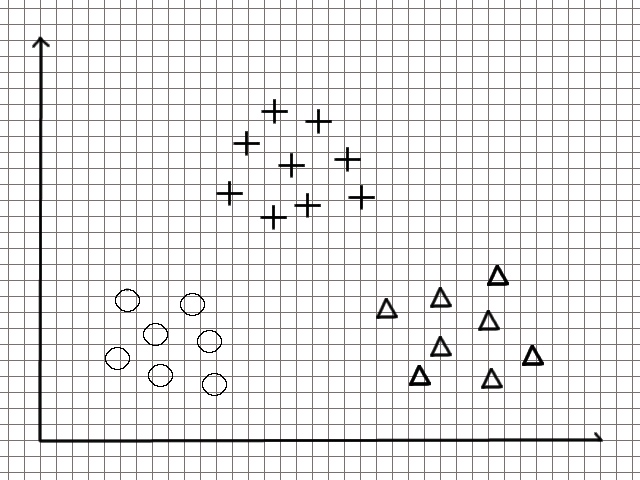
\includegraphics[width=0.75\linewidth]{multiclass_original} 
    \caption{Classes originais} 
    \vspace{4ex}
  \end{subfigure}%% 
  \begin{subfigure}[b]{0.5\linewidth}
    \centering
    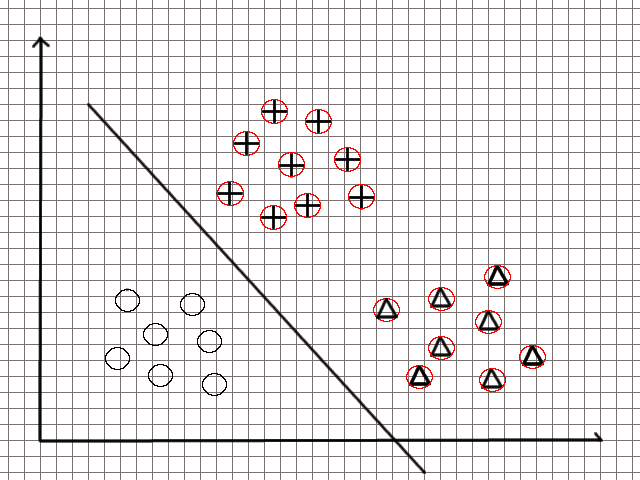
\includegraphics[width=0.75\linewidth]{multiclass_ova1} 
    \caption{Classificador para a classe 1} 
    \vspace{4ex}
  \end{subfigure} 
  \begin{subfigure}[b]{0.5\linewidth}
    \centering
    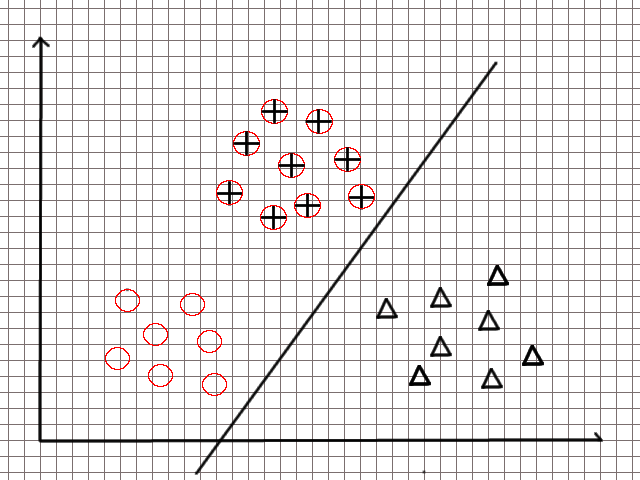
\includegraphics[width=0.75\linewidth]{multiclass_ova2} 
    \caption{Classificador para a classe 2} 
  \end{subfigure}%%
  \begin{subfigure}[b]{0.5\linewidth}
    \centering
    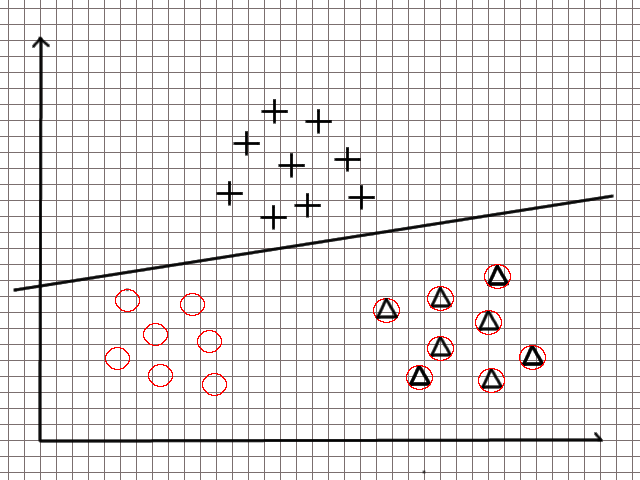
\includegraphics[width=0.75\linewidth]{multiclass_ova3} 
    \caption{Classificaodr para a classe 3} 
  \end{subfigure} 

\end{figure}

\section{Análise de Sentimentos}

O campo de análise de sentimentos, também conhecido como mineração de opinião é uma área da
ciência da computação que analisa as opiniões, sentimentos e atitudes das pessoas em relação
a uma entidade (Bing Liu, 2012)\citep{bingliu2012}. Uma entidade pode ser definida como o sujeito ao qual está
se observando as opiniões, seja ela uma pessoa, instituição ou produto.

A área possui uma diversa gama de aplicações, dentre elas, a área de classificação de sentimentos
que através do uso de informações subjetivas contidas num texto avalia qual a opinião relacionada
ao mesmo.

Classificação de sentimentos teve um crescimento devido à expansão da Web 2.0 que fez com que
as pessoas manifestassem suas opiniões e sentimentos através de blogs, fóruns, redes sociais
e páginas de reviews de produtos que, consequentemente fez com que empresas e pessoas de interesse
tivessem um acesso mais aberto e fácil a essas opiniões. O fácil acesso às opiniões dos usuários
junto com o grande volume delas tornou a análise manual um processo muito custoso, tornando
necessário recorrer a métodos automatizados para a análise e sumarização desses dados que
acabou por fim impulsionando estudos na área (Petković e Ringsquandl, 2013)\citep{petkovic2013}.

Bing Liu (2012)\cite{bingliu2012} divide as formas de classificar sentimentos 
em um documento pode se dividir em quatro formas:
\begin{itemize}
	\item Entidade:  um produto, pessoa sobre o qual o texto se refere, seja direta ou indiretamente.
	Nessa tarefa procura-se analisar se a opinião do texto em torno de uma entidade é positiva ou
	não.
	\item Aspecto: características sobre uma entidade. Por exemplo se temos uma entidade que é um
	produto, aspectos de um produto poderiam ser material ou preço. Nessa forma procura-se avaliar
	a opinião acerca de cada um dos aspectos.
	\item Sentença: esse tipo de análise trabalha com o sentimento associado a cada sentença de
	um documento.
	\item Documento: nesse caso analisa-se o sentimento associado a um documento como um todo, 
	tratando de uma forma mais genérica em relação aos demais.
\end{itemize}

Comum a todas as formas de se analizar as opiniões de um documento é que o uso dos métodos
para obter a opinião. Há duas abordagens para esse problema de classificação: a de aprendizado
de máquina (que iremos utilizar nesse trabalho) que se consiste do uso de algoritmos de 
classificação em conjunto com técnicas de processamento de texto (que será explicado nas próximas
seções) e a abordagem com um dicionário léxico onde a análise é feita baseada na pontuação
entre palavras positivas e negativas contidas no documento (Medhat et al., 2014) \citep{medhat2014}.

No caso desse trabalho, foi escolhido a análise em torno do documento / sentença (devido à estrutura
dos tuítes tem-se que os documentos são, em sua maioria, compostos por apenas uma 
sentença). 

\subsection{Análise de tuítes de política}

Dentre os domínios de aplicação da classificação de sentimentos, escolheu-se como domínio o
escopo político. Nesse caso, temos que as entidades nos documentos são constituídas por
políticos e projetos de lei. E neste trabalho será analisado a análise de tuítes.

O twitter desde as eleições presidenciais estadunidenses de 2008 mostrou influência
na decisão das eleições evidenciado pela campanha online realizada pela equipe do
candidato Barack Obama (Petković e Ringsquandl, 2013)\citep{petkovic2013}. Desde então, 
a rede social tem sido usada não só para a campanha de políticos, mas também para a avaliação
da opinião em relação às medidas tomadas por eles.

A escolha foi feita tendo em vista o uso da rede social 
para expressar opiniões sobre diversos assuntos, incluindo política.


\subsection{Obtendo um vetor de \textit{features}}
\label{subsec:featurization}

Para realizar a extração das informações do texto, existe uma etapa de pré-processamento na qual
cada texto é transformado num vetor numérico para então ser processado por algum algoritmo de
classificação. Neste trabalho foi escolhido usar o modelo \textit{bag of words} (BOW). No modelo, 
é construída uma matriz de entrada onde cada linha i representa um documento (texto sobre o qual
quer extrair a opinião) e as colunas representam a frequência de um termo, o conjunto de todos os textos é chamado de \textit{corpus}.

Uma alternativa ao BOW seria o modelo de N-grama, nele os termos não são apenas as palavras, mas
um conjunto de n palavras juntas, o que traz mais informação pelo fato de juntar substantivo e verbo, substantivo e adjetivo, por exemplo, entretanto acaba gerando um vetor de \textit{features}
ainda maior que, consequentemente, faz com que os algoritmos demorem mais para convergir.
A escolha pelo BOW foi tida baseada no compromisso entre desempenho e performance do algoritmo.

Antes de obter um vetor numérico, é feito um pré-processamento no documento removendo artigos, 
adicionando espaços antes e depois de pontuações e transformando em um vetor de tokens. Uma
vez que foi obtido o vetor de \textit{tokens}, é removido todo elemento que seja apenas espaço e pontuação.
Em seguida, monta-se uma nova \textit{string} juntando todas as \textit{tokens} usando espaços
para então montar um vetor de frequência a partir do novo \textit{corpus}.

A frequência pode ser medidas simples como a quantidade de vezes em que um termo j aparece no documento
i ou se o termo j aparece no documento i (nesse caso cada vetor de entrada seria um vetor binário) bem
como pode ser uma medida mais complexa como tf-idf (\textit{term frequency - inverse document frequency}).
A relação entre os métodos de computar a frequência e o desempenho dos algoritmos de classificação serão
exibidas no capítulo seguinte.

O método tf-idf baseia-se na frequência de cada termo ponderada pela frequência inversa no documento,
que é usada para mensurar o quão importante um termo é em um documento (por exemplo a palavra "um" em
um conjunto de textos em português aparece várias vezes, apesar de ter uma baixa importância).
Ele pode ser calculado pelas expressões:

\begin{center}
	\begin{dgroup}
		\begin{dmath}
			TF(t) = \frac{\text{\# de aparições de t no documento}}{\text{total de termos no documento}} 
		\end{dmath}
		\begin{dmath}
			IDF(t) = log \left(  \frac{\text{Total de documentos}}{\text{\# de documentos que contenham t}} \right) 
		\end{dmath}	    
		\begin{dmath}
			TF-IDF(t) = TF(t)*IDF(t)
		\end{dmath} 	    
	\end{dgroup}
\end{center}

O procedimento de obtenção dos vetores de \textit{features} a partir do novo \textit{corpus} pode
ser realizado utilizando as bibliotecas \texttt{scikit-learn} e \texttt{nltk} do Python.

\subsection{Classificação manual da opinião}

Com o conjunto de dados obtido em \ref{subsec:featurization}, podemos aplicar os algoritmos 
descritos no começo do capítulo. Entretanto como também mencionado no começo deste capítulo,
problemas de aprendizado supervisionado exigem que o conjunto de dados seja composto não só dos
dados, mas também do valor esperado para cada entrada. No caso da classificação da opinião de
textos, tal opinião deve ser primeiro atribuída manualmente para que, com posse dessas opiniões,
seja possível treinar os algoritmos.

Para facilitar a etapa de classificação manual, foi desenvolvido um sistema online onde cada usuário
informa a quantidade de tuítes que se deseja classificar e consegue classificá-los de forma
mais simples. Deu-se a essa ferramenta o nome de CLAM (de Classificador Manual).

O desenvolvimento do CLAM foi motivado pela ausência de ferramentas no Brasil que permitem a
colaboração nessa etapa de classificação manual (uma ferramenta comumente usada é o \textit{Amazon
Mechanical Turk}, porém na época do desenvolvimento do CLAM não estava disponível no Brasil)
em conjunto com a falta de ferramentas gratuitas de 
uma forma geral, uma vez que até que a maioria das ferramentas existentes são pagas (vide o 
próprio \textit{Amazon Mechanical Turk}). Por isso priorizou-se construir um código simples
para que fosse fácil a modificiação da base do sistema por colaboradores externos,
que fosse de fácil uso para o usuário final e também de fácil hospedagem do sistema
em alguma plataforma como Heroku e Firebase.

O código é de domínio público e está disponível no link:
 \url{https://github.com/romaolucas/manual-classifier-helper}

O projeto foi desenvolvido usando a linguagem Python em conjunto do \textit{framework} web
Django por já possuir diversas ferramentas integradas não só de gerenciamento do sistema, bem como
modelagem do banco de dados e sistema de migração para que possa modificar os modelos de dados já
existentes sem precisar realizar um acesso direto à base de dados além de possuir um conjunto
de bibliotecas que facilitam o processo de importação de dados em csv e vasta quantidade de 
tutoriais de como desenvolver uma aplicação usando Django.

Para a modelagem de dados construiu-se dois modelos: um para tuítes e outro para
as opiniões.
Na modelagem, considerou-se que cada usuário irá classificar apenas textos que não 
possuem uma classificação, não só para evitar ter que lidar com opiniões divergentes em um texto,
mas também para garantir um maior número de dados para o treinamento. Uma possível melhoria
do sistema seria a possibilidade de mais usuários avaliarem um mesmo conjunto de textos para
garantir um consenso na hora de associar uma opinião a um texto.

O CLAM possui o seguinte fluxo para a classificação:

\begin{enumerate}
	\item Informa a quantidade de tuítes que se deseja classificar.
	\begin{figure}[H]
		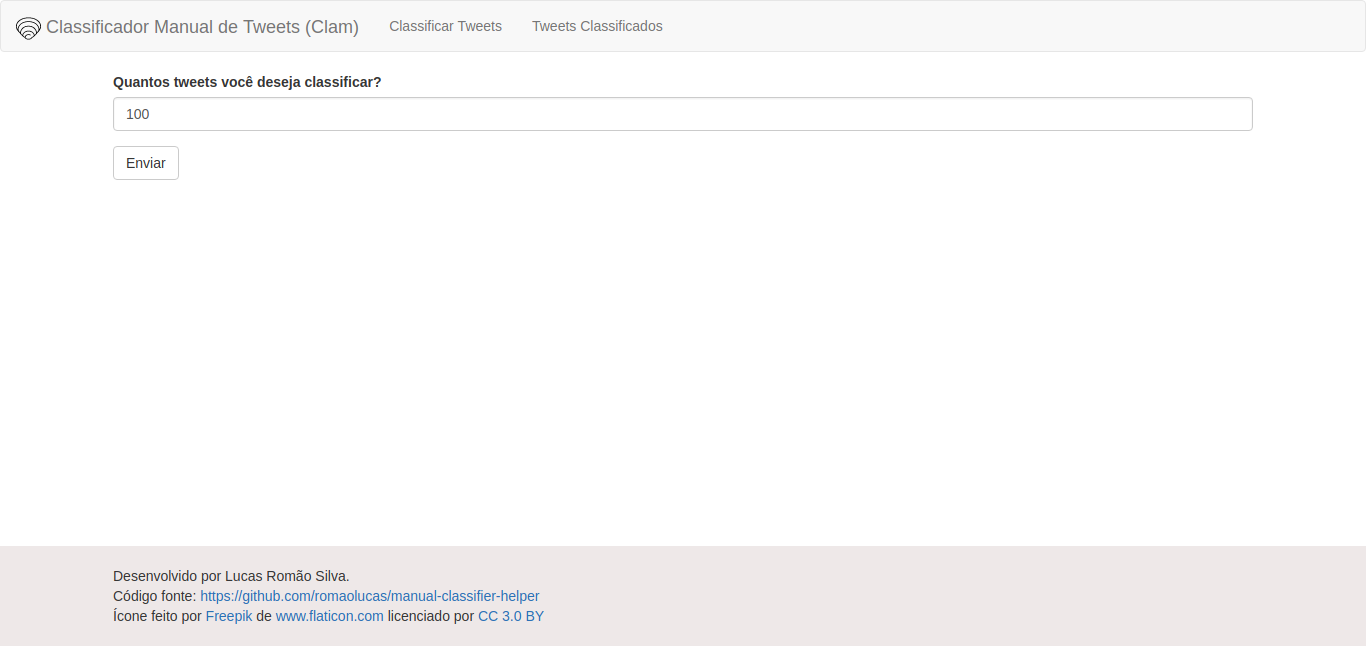
\includegraphics[scale=0.27]{clam_inicio}
	\end{figure}
	\item O usuário é levado a uma página com os n tuítes para classificar.
	Enquanto o campo da opinião é obrigatório, existe um campo optativo para informar
	se o dado tuíte é irônico ou não, uma vez que textos com ironia atrapalham
	o treinamento por conter palavras positivas sendo usadas de maneira negativa e vice-versa.
	\begin{figure}[H]
		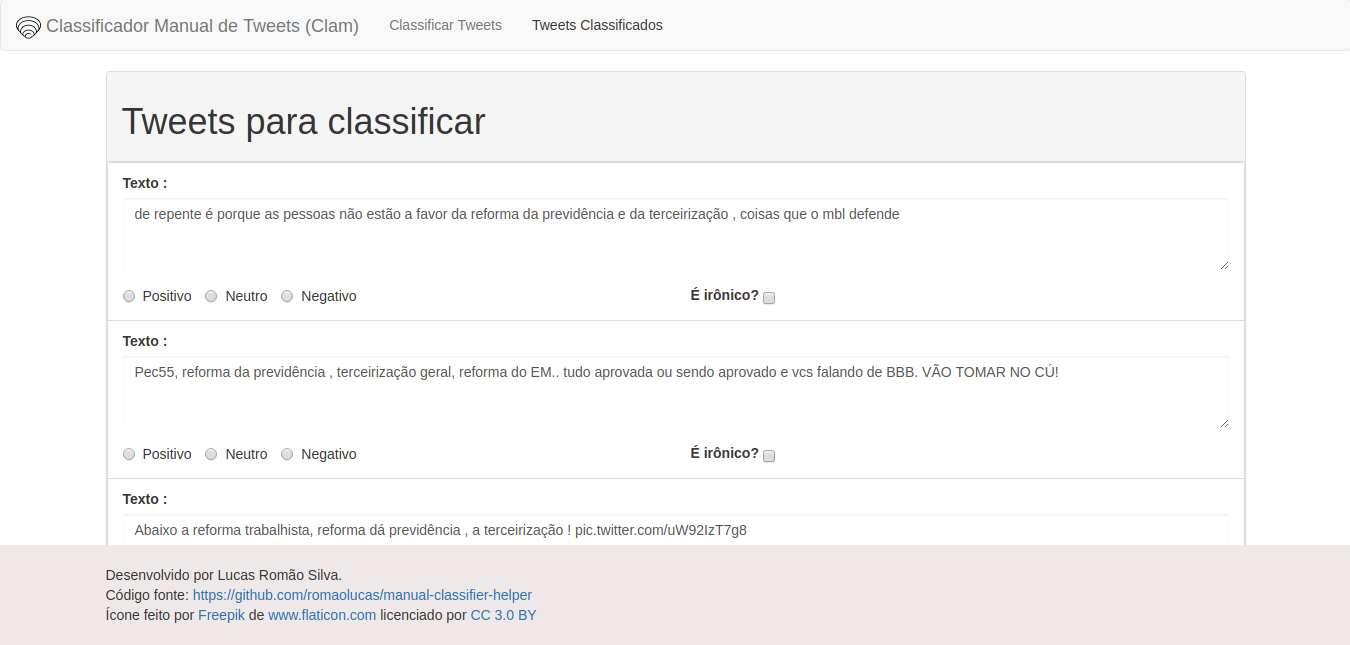
\includegraphics[scale=0.27]{clam_classificar}
	\end{figure}
	\item Uma vez classificados, o usuário é levado a uma página onde é possível ver todos
	os tuítes já classificados e também gerar um arquivo csv contendo todos aqueles
	que não foram marcados como irônicos.
	\begin{figure}[H]
		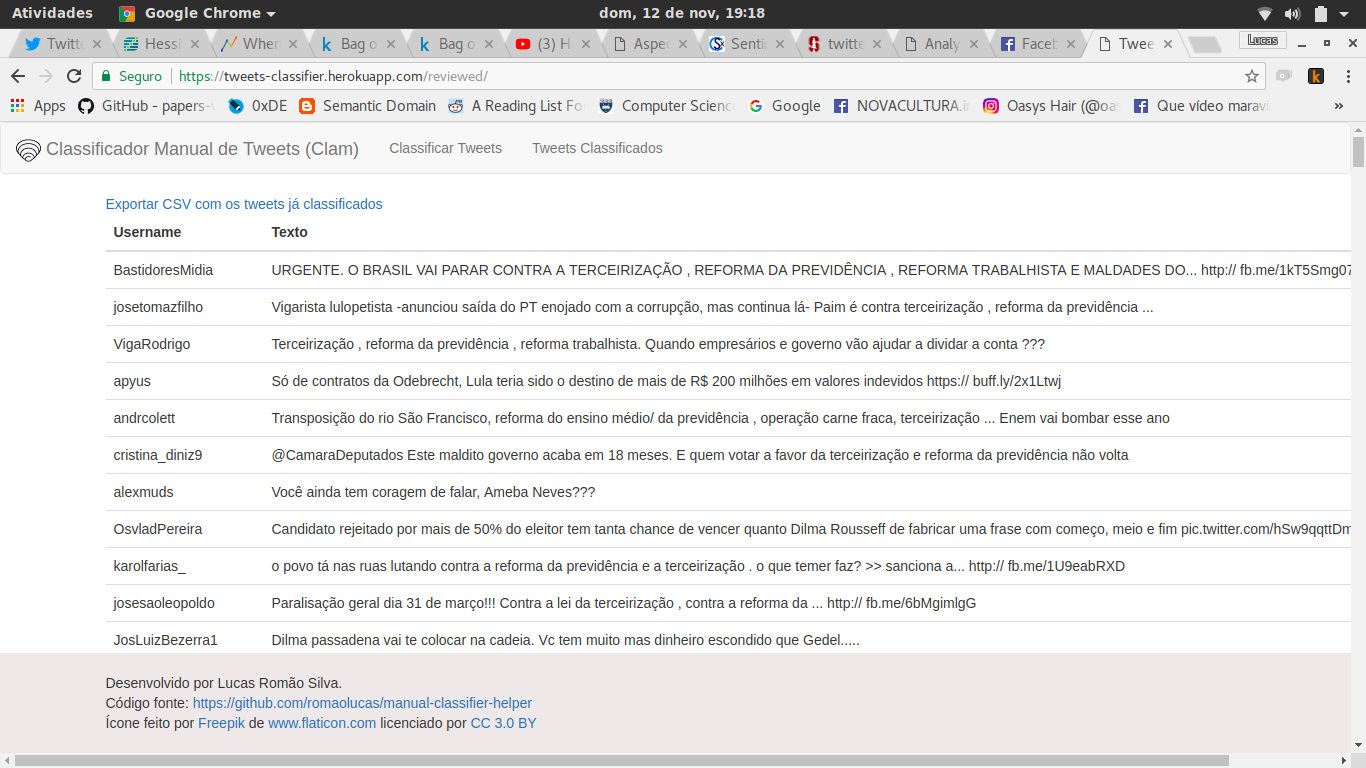
\includegraphics[scale=0.27]{clam_classificados}
	\end{figure}
\end{enumerate}

Para um usuário que deseja hospedar a plataforma e usá-la para si, existe também o admin onde
é possível importar tuítes para serem classificados.

Abaixo é descrito o fluxo para a importação de novos dados no admin.

\begin{enumerate}
	\item Realiza o login no sistema utilizando seu usuário e senha de administrador.
	\begin{figure}[H]
		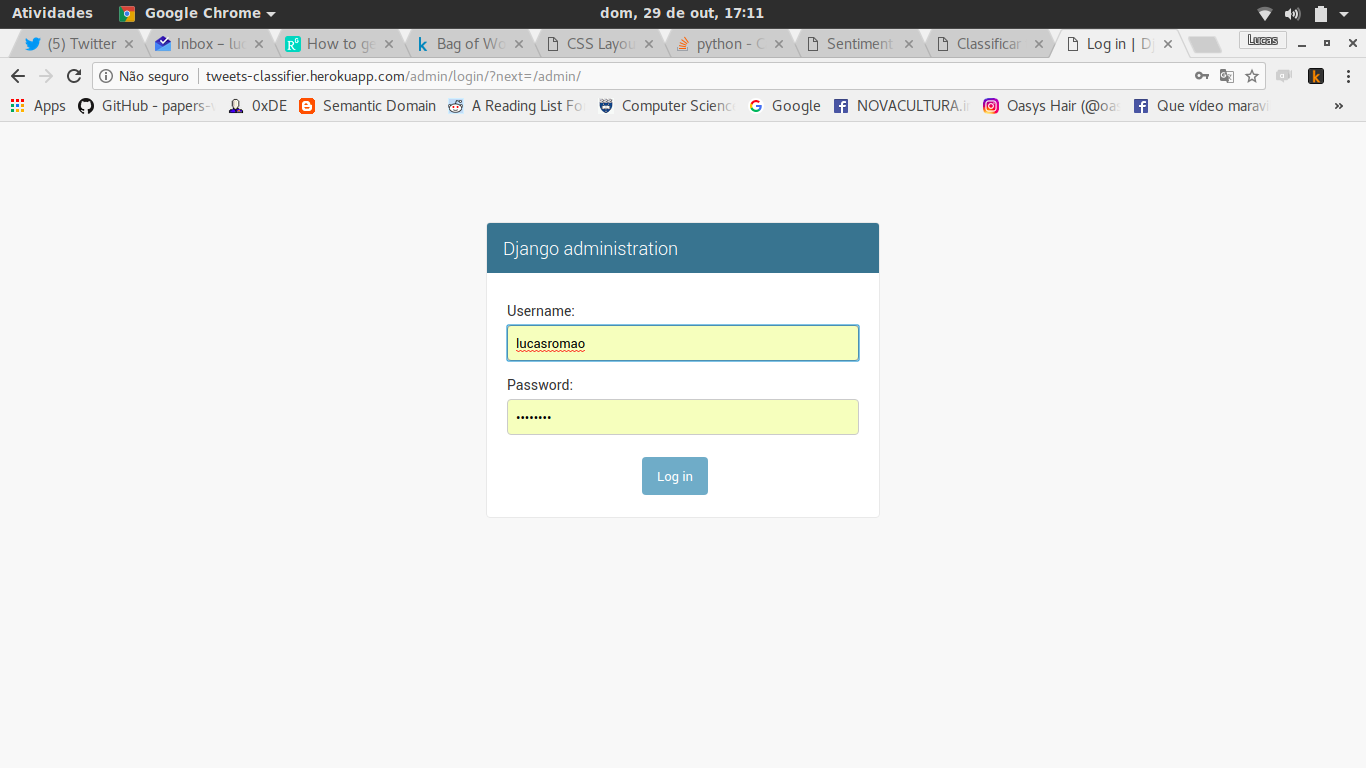
\includegraphics[scale=0.27]{clam_login}
	\end{figure}
	\item Seleciona a parte de Tweets na tela principal.
	\begin{figure}[H]
		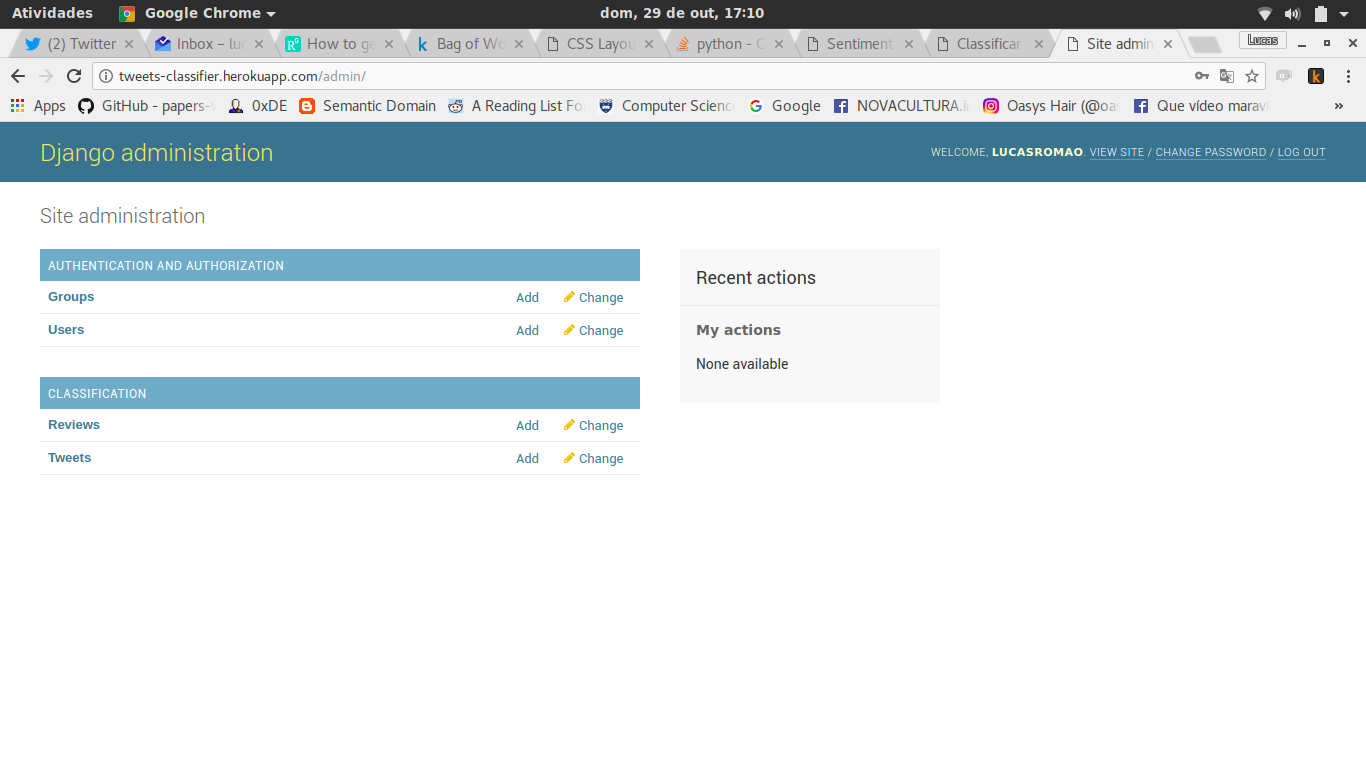
\includegraphics[scale=0.27]{clam_admin}
	\end{figure}
	\item Uma vez na parte de visualizar todos os tuítes já armazenados na base de dados,
	seleciona a opção de importar no canto superior direito.
	\begin{figure}[H]
		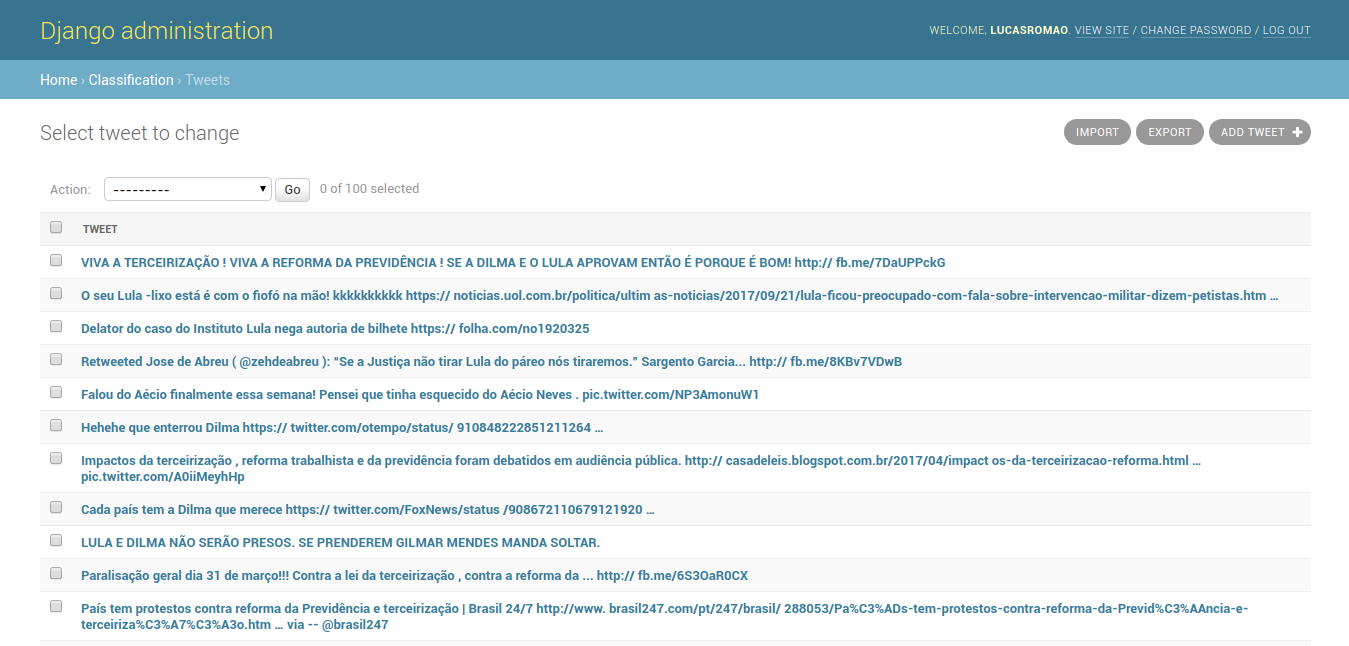
\includegraphics[scale=0.27]{clam_tweets}
	\end{figure}
	\item Na página que segue, basta informar um arquivo .csv, .xls (formato do excel) ou .json
	contendo nessa ordem: o id do tuíte (fornecido pelo Twitter), usuário que escreveu, 
	texto, espaço vazio para representar o id que será preenchido automaticamente na hora de 
	importar no banco de dados.
	\begin{figure}[H]
		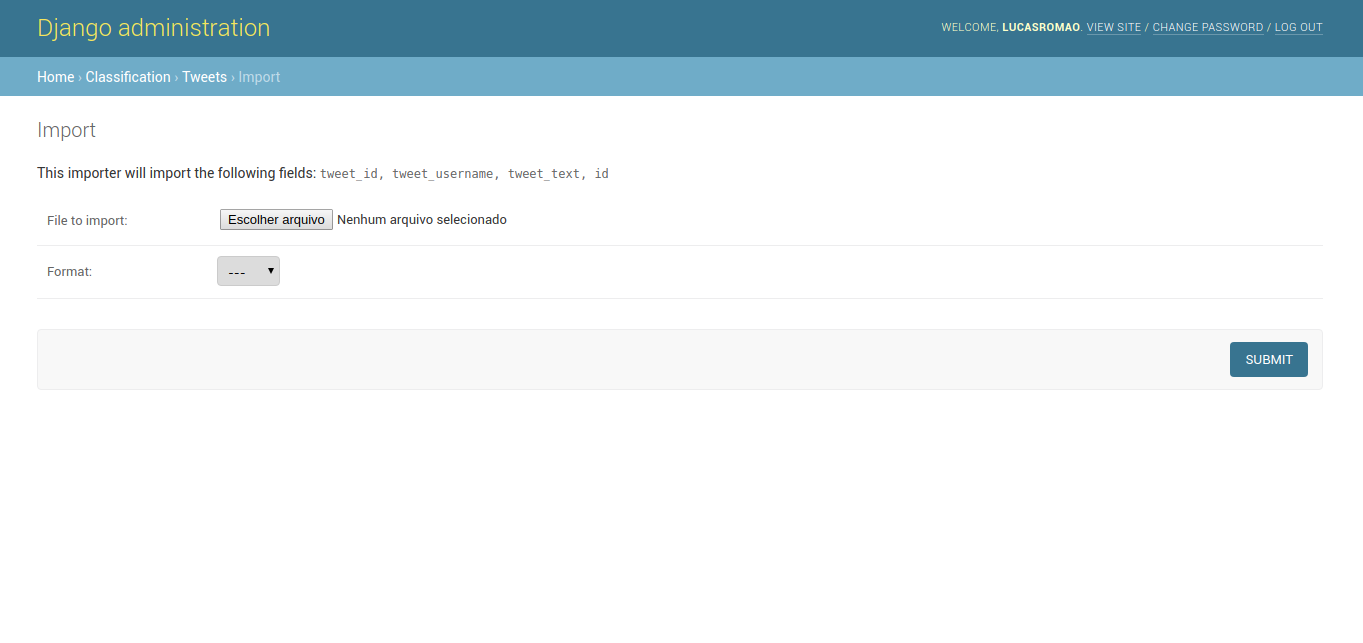
\includegraphics[scale=0.2]{clam_importador}
	\end{figure}
	\item Caso todos os dados sejam fornecidos corretamente, será passado a uma nova página para
	confirmar se deseja importar e, por fim, será redirecionado à pagina que contém todos os
	tuítes.
\end{enumerate}


\chapter{Experimentos}

Uma vez implementado os modelos de classificação, realizou-se experimentos sobre os tuítes
classificados manualmente a fim de encontrar o melhor classificador. Além disso, decidiu-se
comparar os resultados dos classificadores implementados neste trabalho com os já disponíveis
na biblioteca \texttt{scikit} do Python para verificar qual obteria melhores resultados ou se
não haveria diferença.	

Para todos os experimentos, variou-se diversos parâmetros (que serão descritos
em \ref{subsec:parameters}) a fim de encontrar a melhor combinação de parâmetros para cada 
classificador. Essa variação foi feita utilizando a função \texttt{logspace} da biblioteca
\texttt{numpy} que retorna valores igualmente espaçados (numa escala logarítimica) dentro do intervalo 
especificado.

\section{Dataset}

\subsection{Distribuição das classes}

Antes de mais nada, será a composição do conjunto de dados e como se dá
a distribuição de classes. Na figura \ref{fig:classes} tem-se um histograma das classes associadas
a cada tuíte.

\begin{table}[H]
	\begin{center}
		\begin{tabular}{| l | l |}
			\hline
			Classe & Total \\
			\hline
			Positivo & 115 \\
			\hline 
			Negativo & 1248 \\ 
			\hline
			Neutro & 1223 \\ 
			\hline
		\end{tabular}
	\end{center}
	\caption{Quantidade de tuítes pertencentes a cada classe}
	\label{tab:distribution}
\end{table}

\begin{center}
	\begin{figure}[H]
		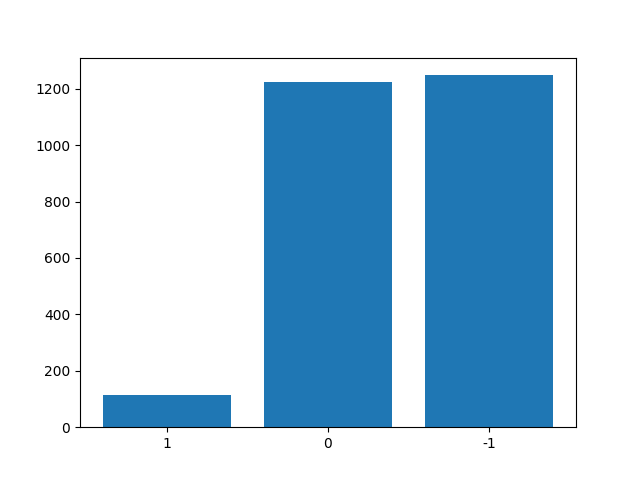
\includegraphics[scale=0.8]{fig_classes}
		\caption{Histograma da frequência de tuítes}
		\label{fig:classes}
	\end{figure}
\end{center}

Pode-se observar nas figura \ref{fig:classes} e tabela \ref{tab:distribution} 
que , ao passo em que as classes negativa e neutra possuem distribuição próxima (48,26\% e 47,29\% 
respectivamente), a classe positiva corresponde a apenas 4,45\% de todos os tuítes. No final da seção
\ref{sec:first_experiments} será visto que esse desbalanceamento entre as classes acarretará um 
desempenho ruim dos classificadores, sejam os desenvolvidos para este trabalho quanto os do
\texttt{scipy}.

\subsection{Características dos tuítes de cada classe}

A fim de entender como os classificadores realizariam o treinamento, analisou-se o conjunto de
dados a procura de padrões de características para cada classe.

Para os tuítes avaliados como neutro, notou-se o padrão que são tuítes derivados de portais de 
notícias ou são indagações, porém sem nenhuma crítica feita nelas.
A tabela abaixo mostra como exemplo alguns tuítes avaliados como neutro.

\begin{center}
	\begin{tabular}{| l | p{0.8\linewidth} |}
		\hline
		usuário & tuíte \\
		\hline
		Tica_Fernandes & Cidades têm protestos contra reforma da Previdência e terceirização http://g1.globo.com/politica/noticia/cidades-tem-protestos-contra-reforma-da-previdência-e-terceirizacao.ghtml \\
		\hline
		andrcolett & Transposição do rio São Francisco, reforma do ensino médio/ da previdência , operação carne fraca, terceirização ... Enem vai bombar esse ano \\
		\hline
		VictoorAugustoo & Via @estadao : Manifestantes protestam em capitais do País contra reforma da Previdência e terceirização - http:/ln.is/estadao.com.brb29w1 \\
		\hline
		EdmilsonPequeno & O meu deputado @luizcoutopt votou contra a terceirização e é contra a reforma da previdência \\
		\hline
	\end{tabular}
\end{center}

Já para os tuítes negativos, nota-se a presença de palavrões e xingamentos 
junto de \textit{hashtags} de teor negativo como por exemplo \#ForaTemer,
além disso é comum a presença de tuítes onde as pessoas são convocadas para manifestações.
Outros termos comuns são escravidão e retrocesso, referindo-se diretamente às reformas da previdência e terceirização.

\begin{center}
	\begin{tabular}{| l | p{0.8\linewidth} |}
		\hline
		usuário & tuíte \\
		\hline
		MgracaGalvao & Dória é o maior Fake de todos os tempos. Se f... Palhaço \\
		\hline
		adamastaquio & Acorda POVO trabalhador. Previdencia + Terceirização + Reforma da CLT é P*** NO RABO DO POVO! \#ReformaTrabalhistaNÃO \\
		\hline
		TheMairaBastos & Reforma da previdência , desmonte da CLT, terceirização ,congelamento de gastos com a saúde e educação \#ForaTemerLadrao \#TemerGolpista \\
		\hline
		neyeverest & O PT esteve no poder por 14 anos o bandido do Lula e a burra da Dilma e o país está um caos pela instituição a roubalheira deles também !! \\
		\hline
		carinasotero & GREVE GERAL DIA 28/04 CONTRA RETROCESSOS DE TEMER • Reforma da Previdência • Reforma Trabalhista • Terceirização irrestrita \\
		\hline
	\end{tabular}
\end{center}

Assim como para os tuítes classificados como negativo, os tuítes positivos também são 
caracterizados pela presença de \textit{hashtags}, sejam elas declarando apoio a um candidato
(como \#Aecio2018 ou \#Lula2018) ou simplesmente manifestando alguma opinião positiva. 

\begin{center}
	\begin{tabular}{| l | p{0.8\linewidth} |}
		\hline
		usuário & tuíte \\
		\hline
		Verinha_Lu & É Aécio pelo Brasil !!! \#AécioPresidenteDoBrasil2018 \#EstamosComAécio \#DeusÉmaior e \#VitóriaVem \#FÉ \#SouAécio \\
		\hline
		Haddad_Femando & O salário mínimo aumentou 71\% durante os governos Lula e Dilma \#BrasilQueOPovoQuer \\
		\hline
		rovisacro & A favor da terceirização e tmb da reforma da previdência ! Mas óbvio, de forma justa e igualitária para todos, principalmente na previdência \\
		\hline	
	\end{tabular}
\end{center}

\section{Descrição dos experimentos}

Realizou-se duas etapas de experimentos, uma primeira etapa utilizando todas as classes onde se
observou que a baixa quantidade de elementos da classe positiva acabava por atrapalhar o desempenho
geral dos algoritmos, em especial os que utilizavam a abordagem OVA para o caso de multiclasses.
Com isso, decidiu-se descartar esses elementos e rodar uma nova sequência de experimentos 
considerando apenas as classes negativa e neutra (que para efeito dos algoritmos será a classe 
positiva) e, com isso, verificar a melhoria dos algoritmos nas métricas.

Para ambas as etapas, procurou-se não só medir o desempenho dos algoritmos, mas também encontrar
uma escolha certa de parâmetros para os mesmos que obtivesse a melhor performance (como a escolha
do Kernel no caso do SVM ou a constante de regularização usada tanto no SVM quanto na regressão
logística).

Tais testes de escolha de parâmetro, caso feitos usando apenas a divisão do conjunto de dados entre
conjunto de treino e conjunto de testes acabaria por dar uma escolha enviesada de parâmetros, uma
vez que uma escolha de parâmetros que tenha bons números em determinado conjunto de testes não
indica que ele possui uma boa generalização, isto é, apresentará uma boa precisão para novos dados.

A fim de garantir maior generalização, utiliza-se um método de validação chamado de 
validação cruzada, que se consiste de um modo de dividir o conjunto de dados e testá-lo com
um conjunto de validação. Uma primeira abordagem da validação cruzada seria dividir nosso conjunto
em três: um de treino, um de validação e outro de teste, assim testaríamos as escolhas de parâmetros
no conjunto de validação e, por fim, mediríamos a performance do melhor no conjunto de teste.

Outra abordagem seria ainda manter a divisão do conjunto de dados em conjunto de treino e teste
porém realizar esse procedimento diversas vezes alternando as porções que irão corresponder a
cada conjunto. Tal método é chamado de k-fold. No k-fold divide-se o conjunto total em k partições
e, a cada iteração, é construído um conjunto de teste usando uma das partições enquanto as k-1
serão o de treino. O procedimento de treinamento é realizado k vezes e, a escolha de parâmetros
com melhor desempenho médio será a escolhida. A figura \ref{fig:kfold} mostra o funcionamento do
método.

\begin{figure}[H]
	\begin{center}
		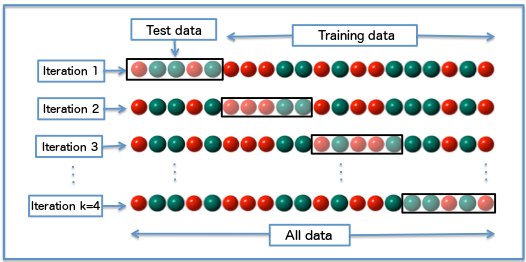
\includegraphics[scale=0.8]{K-fold_cross_validation}
	\end{center}		
	\caption{Funcionamento do método k-fold da validação cruzada \\
		fonte: \url{https://en.wikipedia.org/wiki/Cross-validation_(statistics)\#/media/File:K-fold_cross_validation_EN.jpg}}
	\label{fig:kfold}
\end{figure}

Outro procedimento que foi analisado nos experimentos é se as diferentes escolhas de vetorização afetam
as métricas (ver \ref{subsec:metrics}), todavia esse procedimento de vetorização é feito antes 
do treinamento dos modelos e portanto não foi variado no procedimento de Cross-Validation. 
Em \ref{sec:first_experiments} e \ref{sec:second_experiments} 
os resultados são separados por vetorização e, ao fim de cada rodada, explica-se os resultados 
observados.

O fluxo da realização dos experimentos é descrita no diagrama abaixo:

\begin{figure}[H]
\label{fig:diagram}
	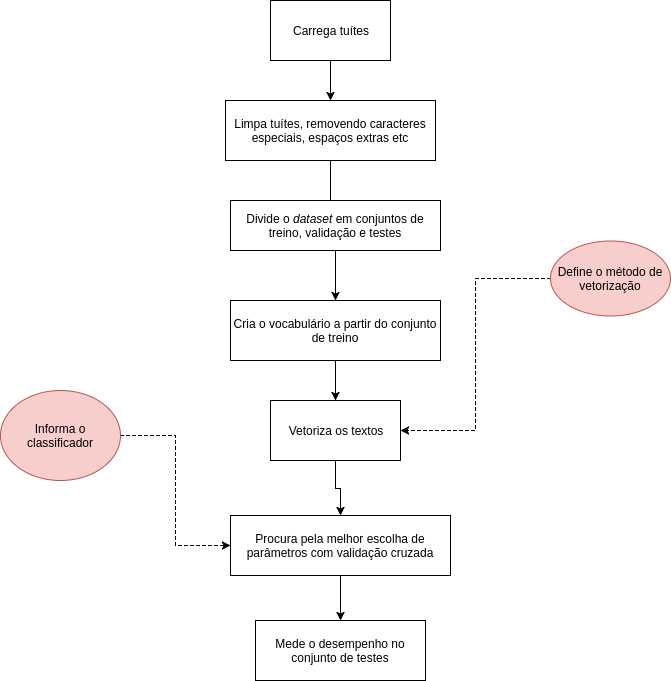
\includegraphics[scale=0.5]{experimento_flow}
	\caption{Passos dos experimentos}
\end{figure}

\subsection{Parâmetros avaliados}
\label{subsec:parameters}

\textbf{SVM}

Para o SVM, testou-se o desempenho do algoritmo com diferentes kernels e com diferentes
parâmetros para cada um. Os seguintes kernels foram utilizados:

\begin{itemize}
	\item Kernel Linear: $K(x, y) = x^Ty$
	\item Kernel RBF: $K(x, y) = exp(-\gamma||x - y||^2)$
	\item Kernel Polinomial: $K(x, y) = (x^Ty + c)^d$
\end{itemize}

Em comum a todos os kernels, variou-se o parâmetro C do SVM utilizado para penalizar os valores
mal classificados. Já para o RBF, varia-se o parâmetro $\gamma$. Por último para o polinomial,
varia-se tanto o parâmetro d que determina o grau do polinômio (aqui variamos entre 3, 4 e 5) e o coeficiente.

\textbf{Regressão Logística}

Para a regressão logística, adicionamos um parâmetro extra $\lambda$ que será usado para penalizar
nosso vetor de pesos e assim, evitar \textit{overfitting}, que ocorre quando um modelo apresenta
baixo erro no conjunto de treino, porém baixa generalização. 
Importante ressaltar que $\lambda$ só é aplicado nos índices
de $1$ a $m + 1$ do vetor de pesos, com o valor do termo $w_0$ não sendo penalizado.


\subsection{Métricas avaliadas}
\label{subsec:metrics}

Para a realização dos experimentos, levou-se em consideração quatro métricas
para avaliar a eficiência dos classificadores.

\begin{itemize}
	\item Acurácia: taxa calculada pela quantidade de dados corretamente classificados
	sobre o total de dados. Quanto mais próximo de 1, melhor.
	\item Precisão: taxa calculada pela expressão $\frac{tp}{tp + fp}$ onde tp corresponde
	aos verdadeiro positivos, isto é, elementos corretamente classificados como da classe C
	e fp são elementos erroneamente classificados na classe C. Uma classe ter precisão alta
	significa que possui um baixo número de amostras classificadas erroneamente nela.
	\item Revocação: taxa calculada pela expressão $\frac{tp}{tp + fn}$ onde tp corresponde
	aos verdadeiro positivos, como na precisão e fn corresponde
	aos falso negativos, isto é, os elementos incorretamente classificados como não pertencentes
	a uma classe C quando na verdade pertencem. Uma alta revocação indica que muitos elementos
	de determinada classe foram corretamente classificados como pertencentes a ela.
	\item Pontuação F1: pode ser interpretado como uma média harmônica entre precisão e revocação é dado
	pela expressão: $2*\frac{precis*revocação}{precis + revocação}$. Assim como as demais medidas, quanto
	mais próximo de 1, melhor o valor.
\end{itemize}

\section{Primeira rodada de experimentos}
\label{sec:first_experiments}

Nesse primeiro experimento, avaliou-se o desempenho dos classificadores desenvolvidos quanto dos
já disponíveis pela biblioteca \texttt{scikit} a fim de comparar o desempenho das implementações.
Além disso, testou-se diferentes escolhas de parâmetro para cada abordagem de vetorizar o corpus
que no caso foram vetor binário, vetor de frequência e vetor com os valores tf-idf conforme descrito
em \ref{subsec:featurization}. 
Note que neste primeiro experimento, todos os dados foram tratados \textit{in-natura}, sem nenhum método de seleção de características ou qualquer abordagem semelhante a fim de melhorar o desempenho.

\subsection{Implementações próprias}

Dos algoritmos desenvolvidos neste trabalho, testou-se o SVM variando o valor de C entre valores
do intervalo $[10^{-2}, 10^5]$, kernels polinomial, RBF e linear. Para o kernel polinomial foi utilizado
polinômios de grau 3, 4 e 5 e coeficientes 1, 10 e 100. Para o kernel RBF testou valores de $\gamma$
dentro do intervalo $[10^{-9}, 10^3]$. Para cada escolha de vetorização, será colocado apenas os
melhores resultados para cada kernel.

\textbf{Frequência}

\begin{table}[H]
	\centering
	\caption{Resultados para o SVM}
	\begin{tabular}{l l l l}
		\hline
		Kernel & C & parâmetros & Acurácia média \\
		\hline
		Linear & 0,1 & & 0,678 \\
		\hline
		Linear & 1 & & 0,651 \\
		\hline
		RBF & 1 & $\gamma = 0,1$ & 0,683 \\
		\hline
		RBF & $10^5$ & $\gamma = 4,64*10^{-7}$ & 0,678 \\
		\hline
	\end{tabular}
\end{table}

A escolha de parâmetros que obteve maior classificação foi o kernel RBF com C = 1 e $\gamma = 0,1$
com acurácia média de 68,3\%. Usando o classificador com estes parâmetros no conjunto de testes
obteve-se o seguinte resultado:

\begin{table}[H]
	\centering
	\begin{tabular}{l | l | l | l | l}
		\hline
		classe  	&	precisão  &  revocação &  f1\-score &  support \\
		\hline
         -1   &    0.65  &    0.66   &   0.66   &    306 \\
         \hline
          0   &    0.64   &   0.69   &   0.67    &   311 \\
          \hline
          1   &    1.00   &   0.03   &   0.06    &    30 \\
		\hline
		média / total   &    0.67   &   0.65   &   0.64   &    647 \\
		\hline
	\end{tabular}
\end{table}

\textbf{Vetor binário}

\begin{table}[H]
	\centering
	\caption{Resultados para o SVM}
	\begin{tabular}{l l l l}
		\hline
		Kernel & C & parâmetros & Acurácia média \\
		\hline
		Linear & 0,146 & & 0,675 \\
		\hline
		Linear & 0,563 & & 0,658 \\
		\hline
		RBF & 2,154 & $\gamma = 0,1$ & 0,677 \\
		\hline
		RBF & 464,16 & $\gamma = 4,64*10^{-7}$ & 0,676 \\
		\hline
		Polinomial & 0,01 & $c = 1$, $d = 3$ & 0,641 \\
		\hline
		Polinomial & 0,01 & $c = 1$, $d = 3$ & 0,642 \\
		\hline
	\end{tabular}
\end{table}

Como melhor escolha de parâmetros, tivemos o kernel RBF com C = 464,16 e $\gamma = 0,1$ com
67,7\% de acurácia. Utilizando os parâmetros no conjunto de testes, obteve-se os seguintes
resultados:

\begin{table}[H]
	\centering
	\begin{tabular}{l | l | l | l | l}
		\hline
		classe  	&	precisão  &  revocação &  f1\-score &  support \\
		\hline
         -1   &    0.69  &    0.72   &   0.70   &    307 \\
         \hline
          0   &    0.70   &   0.72   &   0.71    &   315 \\
          \hline
          1   &    1.00   &   0.08   &   0.15    &    25 \\
		\hline
		média / total   &    0.71   &   0.70   &   0.69   &    647 \\
		\hline
	\end{tabular}
\end{table}

\textbf{Tf-idf}

\begin{table}[H]
	\centering
	\caption{Resultados para o SVM}
	\begin{tabular}{l l l l}
		\hline
		Kernel & C & parâmetros & Acurácia média \\
		\hline
		Linear & 0,146 & & 0,651 \\
		\hline
		Linear & 0,563 & & 0,664 \\
		\hline
		RBF & 1778,279 & $\gamma = 2,15*10^{-4}$ & 0,667 \\
		\hline
		RBF & 26101,572 & $\gamma = 10^{-5}$ & 0,666 \\
		\hline
		Polinomial & 0,038 & $c = 1$, $d = 4$ & 0,660 \\
		\hline
		Polinomial & 0,147 & $c = 1$, $d = 3$ & 0,663 \\
		\hline
	\end{tabular}
\end{table}

Assim como as demais escolhas de vetorização, a melhor escolha de kernel foi o RBF.
Com valor de C = 1778,279 e $\gamma = 2,15*10^{-4}$ conseguiu-se acurácia média de 66,7\%.
Utilizando esse classificador no conjunto de testes, obtiveram-se os seguintes resultados:

\begin{table}[H]
	\centering
	\begin{tabular}{l | l | l | l | l}
		\hline
		classe  	&	precisão  &  revocação &  f1\-score &  support \\
		\hline
         -1   &    0.68  &    0.73   &   0.70   &    322 \\
         \hline
          0   &    0.67   &   0.69   &   0.68    &   296 \\
          \hline
          1   &    1.00   &   0.03   &   0.07    &    29 \\
		\hline
		média / total   &    0.69   &   0.68   &   0.66   &    647 \\
		\hline
	\end{tabular}
\end{table} 

Pelos resultados dos experimentos, tivemos que a melhor escolha de classificador e vetorização
foi o kernel RBF com vetorização por frequência com 68,3\% de acurácia. Ao observarmos as outras
métricas, percebemos que os valores médios para precisão, revocação e pontuação f1 estão razoáveis,
entretanto ao olharmos para os valores de revocação e pontuação f1 da classe positiva, vemos
que estes são quase 0 ao passo que a precisão é 1. Isso indica que apenas poucos elementos foram
colocados nesta classe corretamente e nenhum foi colocado incorretamente, porém a maioria dos
elementos desta classe foram marcados nas demais classes.

Tais valores para classe positiva são devidos à baixa quantidade de dados da mesma, o que acaba
prejudicando o desempenho do classificador que separa esta classe das demais.

Utilizou-se o melhor classificador para verificar alguns tuítes mal classificados e entender melhor
o funcionamento do classificador.

\begin{table}[H]
	\centering	
	\begin{tabular}{| p{0.8\linewidth} | l | l |}
		\hline
		Tuíte & Previsto & Real \\
		O cara tá falando da terceirização anta. Eu sou contra essa reforma da previdência deste jeito, ela deve ser revista.A trabalhista eu apoio & -1 &  1 \\
		\hline
		Ops @MichelTemer não tem um papel com os trabalhadores e a lei da terceirização assim fala os especialistas imagina essa REFORMA PREVIDÊNCIA  http://pic.twitter.com/KjLa26TCwy &  -1 & 0 \\
		\hline
		A agenda do Lula para os próximos meses está lotada... de depoimentos em processos em que ele é réu. http://owl.li/F3Ij30flUaY & 0 & -1 \\
		\hline
		Contra reforma da Previdência e terceirização ... http://fb.me/18guG6FGR & 0 & -1 \\
		\hline
		Não podemos discutir a Reforma da Previdência sem discutir a Terceirização e outros elementos desse desmonte de direitos", Ruy (APLB)" & -1 & 0 \\
		\hline
		Muso inspirador da presidenta Dilma ! & 0 & 1 \\
		\hline
	\end{tabular}
\end{table} 

Para os tuítes negativos que foram erroneamente classificados, percebemos que o classificador os
colocou na classe neutra pela maior presença de palavras encontradas em tuítes de notícias, no segundo
caso percebe-se que há uma ambiguidade no tuíte e, enquanto foi classificado com negativo, poderia
ter sido também classificado como neutro por outra pessoa.

Na classe neutra, temos que em um há uma ambiguidade no tuíte e não possui informação suficiente
para avaliar sua polaridade, porém no segundo caso pode-se dizer que o tuíte foi classificado corretamente
pois o classificador levou em conta que chamou a reforma de previdência e a terceirização de desmonte
de direitos, apesar de o tuíte em si apenas relatar o que foi dito.

Para a classe positiva notou-se dois casos: em um a presença de um xingamento colocou o tuíte como
opinião negativa e no outro caso o classificador interpretou o tuíte como uma simples constatação
de fatos.


\subsection{Implementações do \texttt{scikit}}

Abaixo, separaremos os testes baseados em como a obtenção do vetor de \textit{features} foi feita
ao invés dos algoritmos, uma vez que para todos esses realizou-se os mesmos testes. Importante 
ressaltar que só serão colocados aqui os melhores resultados de cada um, uma vez que existe uma
grande quantidade de resultados. 

Os resultados dos experimentos serão comentados apenas ao final desta subseção, após mostrar
os valores encontrados para todas as formas de vetorização.


\textbf{Frequência}

\begin{table}[H]
	\centering
	\caption{Resultados para o SVM}
	\begin{tabular}{l l l l}
		\hline
		Kernel & C & parâmetros & Acurácia média \\
		\hline
		Linear & 0,1 & & 0,666 \\
		\hline
		Linear & 1 & & 0,637 \\
		\hline
		RBF & 100 & $\gamma = 10^{-3}$ & 0,663 \\
		\hline
		RBF & 100 & $\gamma = \frac{1}{\# amostras}$ & 0,653 \\
		\hline
		Polinomial & 0,01 & $c = 10$, $d = 5$ & 0,666 \\
		\hline
		Polinomial & 100 & $c = 1$, $d = 4$ & 0,663 \\
		\hline
	\end{tabular}
\end{table}

Importante ressaltar que em casos de empate, o primeiro melhor será selecionado, no caso o melhor
foi o kernel linear com $C = 0.1$, utilizando esses valores no conjunto de testes obtiveram-se os 
seguintes resultados:

\begin{table}[H]
	\centering
		\begin{tabular}{l | l | l | l | l}
		\hline
		classe  	&	precisão  &  revocação &  f1\-score &  support \\
		\hline		
		 -1     &  0.70  &    0.73   &   0.71   &    324 \\
		  \hline
          0     &  0.67   &   0.69   &   0.68    &   298 \\
          \hline
          1     &  1.00   &   0.04   &   0.08    &    25 \\
			\hline
		média / total     &  0.70  &    0.68  &    0.67   &    647 \\
		\hline
	\end{tabular}
\end{table}

Para a regressão logística, variou-se o valor de $\lambda$ entre $10^{-4}$ a $1$ e, além disso
variou-se a abordagem para o caso multiclasses, uma vez que o \texttt{scikit} disponibiliza
uma implementação usando o método OVA e outro usando o método multinomial (assim como implementou-se).

\begin{table}[H]
	\centering
	\caption{Resultados da regressão logística}
	\begin{tabular}{l l l}
		\hline
		Método & $\lambda$ & Acurácia média \\
		\hline
		OVA & 0.1 & 0.654 \\
		\hline
		OVA & 1 & 0.651 \\
		\hline
		Multinomial & 0.1 & 0.654 \\
		\hline
		Multinomial & 1 & 0.649 \\
		\hline
	\end{tabular}
\end{table}

Assim como para o SVM, escolheu-se o primeiro melhor que no caso é a abordagem OVA com $\lambda = 0.1$.
Deu os seguintes resultados no conjunto de testes:

\begin{table}[H]
	\centering
		\begin{tabular}{l | l | l | l | l}
		\hline
		classe  	&	precisão  &  revocação &  f1\-score &  support \\
		\hline
         -1   &    0.70  &    0.68   &   0.69   &    320 \\
         \hline
          0    &   0.68   &   0.73   &   0.70   &    307 \\
          \hline
          1    &   0.50   &   0.15   &   0.23   &     20 \\
		\hline
		média / total  &     0.68  &    0.69    &  0.68   &    647 \\
		\hline
	\end{tabular}
\end{table}

\textbf{Vetor binário}

\begin{table}[H]
	\centering
	\caption{Resultados para o SVM}
	\begin{tabular}{l l l l}
		\hline
		Kernel & C & parâmetros & Acurácia média \\
		\hline
		Linear & 0,1 & & 0,658 \\
		\hline
		Linear & 1 & & 0,643 \\
		\hline
		RBF & 100 & $\gamma = 10^{-3}$ & 0,649 \\
		\hline
		RBF & 100 & $\gamma = \frac{1}{\# amostras}$ & 0,646 \\
		\hline
		Polinomial & 100 & $c = 1$, $d = 4$ & 0,656 \\
		\hline
		Polinomial & 1 & $c = 5$, $d = 4$ & 0,658 \\
		\hline
	\end{tabular}
\end{table}

Assim como para o vetor de frequências, a melhor escolha de parâmetros encontrada na validação
cruzada foi C = 0,1 e kernel linear. Executando no conjunto de testes obtiveram-se os seguintes
resultados:

\begin{table}[H]
	\centering
		\begin{tabular}{l | l | l | l | l}
		\hline
		classe  	&	precisão  &  revocação &  f1\-score &  support \\
		\hline
         -1    &   0.66   &   0.76  &    0.71    &   310 \\
         \hline
          0     &  0.69   &   0.66   &   0.67    &   302 \\
         \hline
          1     &  1.00  &    0.06   &   0.11    &    35 \\
		\hline
		média / total    &   0.69   &   0.68   &   0.66    &   647 \\
		\hline
	\end{tabular}
\end{table}

\begin{table}[H]
	\centering
	\caption{Resultados da regressão logística}
	\begin{tabular}{l l l}
		\hline
		Método & $\lambda$ & Acurácia média \\
		\hline
		OVA & 0.1 & 0.631 \\
		\hline
		OVA & 1 & 0.634 \\
		\hline
		Multinomial & 0.1 & 0.631 \\
		\hline
		Multinomial & 1 & 0.630 \\
		\hline
	\end{tabular}
\end{table}

Tal qual com o vetor de frequências, escolheu-se a abordagem OVA e $\lambda = 1$ obtendo os seguintes
resultados no conjunto de testes:

\begin{table}[H]
	\centering
		\begin{tabular}{l | l | l | l | l}
		\hline
		classe  	&	precisão  &  revocação &  f1\-score &  support \\
		\hline
		 -1    &   0.68   &   0.73  &    0.71   &    305 \\
		 \hline
          0    &   0.70   &   0.69   &   0.69   &    317 \\
          \hline
          1   &    0.33   &   0.04   &   0.07   &     25 \\
		 \hline
		média / total    &   0.67   &   0.69  &    0.68   &    647 \\
		\hline
	\end{tabular}
\end{table}

\textbf{Tf-idf}

\begin{table}[H]
	\centering
	\caption{Resultados para o SVM}
	\begin{tabular}{l l l l}
		\hline
		Kernel & C & parâmetros & Acurácia média \\
		\hline
		Linear & 1 & & 0,658 \\
		\hline
		Linear & 10 & & 0,627 \\
		\hline
		RBF & 100 & $\gamma = 10^{-3}$ & 0,651 \\
		\hline
		RBF & 1 & $\gamma = 10^{-4}$ & 0,483 \\
		\hline
		Polinomial & 1 & $c = 5$, $d = 5$ & 0,678 \\
		\hline
		Polinomial & 10 & $c = 10$, $d = 3$ & 0,677 \\
		\hline
	\end{tabular}
\end{table}

Com essa vetorização, diferente das demais, os melhores parâmetros escolhidos foram kernel polinomial
com coeficiente e grau 5. Utilizando esses valores, obtiveram-se o seguinte resultado no conjunto de
testes:

\begin{table}[H]
	\centering
		\begin{tabular}{l | l | l | l | l}
		\hline
		classe  	&	precisão  &  revocação &  f1\-score &  support \\
		\hline
		 -1    &   0.64   &   0.79   &   0.71   &    311 \\
		 \hline
          0    &   0.69   &   0.60  &    0.64    &   301 \\
          \hline
          1   &    0.00   &   0.00   &   0.00    &    35 \\
          \hline
		média / total   &    0.63   &   0.66   &   0.64   &    647 \\
		\hline
	\end{tabular}
\end{table}

\begin{table}[H]
	\centering
	\caption{Resultados da regressão logística}
	\begin{tabular}{l l l}
		\hline
		Método & $\lambda$ & Acurácia média \\
		\hline
		OVA & 0.1 & 0.659 \\
		\hline
		OVA & 1 & 0.665 \\
		\hline
		Multinomial & 0.1 & 0.660 \\
		\hline
		Multinomial & 1 & 0.662 \\
		\hline
	\end{tabular}
\end{table}

Neste teste, assim como os demais usando a regressão logística, escolheu-se a abordagem OVA com
$\lambda = 1$ obtendo seguintes resultados no conjunto de testes:

\begin{table}[H]
	\centering
		\begin{tabular}{l | l | l | l | l}
		\hline
		classe  	&	precisão  &  revocação &  f1\-score &  support \\
		\hline
		 -1    &   0.66   &   0.75   &   0.70   &    312 \\
		 \hline
          0    &   0.69   &   0.66   &   0.68   &    310 \\
          \hline
          1    &   0.00   &   0.00   &   0.00    &    25 \\
		\hline
		média / total   &    0.65   &   0.68   &   0.66   &    647 \\
		\hline
	\end{tabular}
\end{table}

Observa-se que, para ambos os algoritmos tem-se que nenhum valor foi classificado como
positivo quando usou-se a vetorização através do valor tf-idf de cada termo, apesar de ainda
apresentar desempenho médio aceitável. 

Isso se deve ao fato de vetorização por tf-idf
leva-se em consideração a relevância das palavras na sentença como um todo e, possivelmente
algumas palavras associadas a documentos positivos estão também associadas
a documentos neutros e, consequentemente, não possuem um valor tf-idf alto, aliado ao fato de o vocabulário
ser montado levando em conta apenas as 5000 palavras com melhores pontuações ou presença, portanto
algumas palavras explicitamente associadas a documentos positivos não compuseram o vetor de
\textit{features}.

Por outro lado se olharmos os desempenhos utilizando frequências simples ou um vetor binário
obtemos resultados semelhantes para ambos os algoritmos, todavia ainda existe um melhor desempenho
com a vetorização por frequências tal como o SVM apresenta melhores resultados em relação à regressão
logística, mesmo que com pouca diferença.

Assim como o outro classificador, analisou-se os tuítes classificados incorretamente a fim de
entender o funcionamento do classificador:

\begin{table}[H]
	\centering
	\begin{tabular}{| p{0.8\linewidth} | l | l |}
		\hline
		Tuíte & Previsto & Real \\
		\hline
		Lula ainda lidera as pesquisas oficiais em todo o Brasil & -1 & 0 \\
		\hline
		Sem querer ser chata, mas foi a Dilma quem começou com os Projetos de Reforma da Previdência e de Terceirização & -1 & 0 \\
		\hline
		simm, e irei, quero a reforma da previdência , a terceirização , reforma da CLT, tudo isso p o Brasil voltar a crescer :) & -1 & 1 \\
		\hline
		O cara tá falando da terceirização anta. Eu sou contra essa reforma da previdência deste jeito, ela deve ser revista.A trabalhista eu apoio & -1 & 1 \\
		\hline
		Temer não é santo,mas não entender o conceito que deu uma freada na beira do abismo que Lula Dilma estavam nos empurrando é DESINFORMAÇÃOhttps://twitter.com/Acppprovesi/status & 0 & -1 \\
		\hline
		Texto: Os alunos da FDCE se posicionam CONTRA a reforma da previdência , trabalhista e a terceirização ! Quem é de luta e... http://fb.me/1YA1jro5z & 0 & -1 \\
		\hline
	\end{tabular}
\end{table}

Observa-se na tabela, assim como para as implementações próprias, houve a classificação errada
de tuítes positivos como negativos devida à presença de xingamentos no tuíte. Além disso tuítes
negativos costumam ser classificados erroneamente como neutros pelo texto se assemelhar com uma
constatação de um fato, mesmo que possua a presença de termos negativos.

Comum a todos os experimentos foram resultados ruins associados à classe positiva. No caso do SVM
obtiveram-se alta precisão em alguns casos, porém as taxas de revocação e f1-score foram baixas. Valores
baixos para revocação e f1-score podem ser interpretados como um sinal de que os classificadores
são ruins para detectar opiniões positivas. A exemplo do melhor classificador, tem-se uma taxa
de revocação de 0,08 que indica que 92\% das amostras positivas não são detectadas pelo algoritmo.

Motivado pelo baixo desempenho visto na classe positiva em todos os experimentos aliado à baixa
quantidade de tuítes nessa classe, rodou-se mais experimentos, porém dessa vez usando apenas as
outras classes.

\section{Segunda rodada de experimentos}
\label{sec:second_experiments}

Nesta segunda rodada de experimentos, removeu-se os elementos pertencentes à classe positiva.
Assim como na primeira rodada, testou-se diferentes escolhas de parâmetros para cada um dos
algoritmos e testou-se com os dados \textit{in natura}. Como viu-se na primeira rodada de experimentos
que havia pouca diferença entre a vetorização por frequência e presença do termo, optou-se por testar
apenas usando frequência e tf-idf.

\subsection{Implementações próprias}

Para as implementações próprias do SVM, testou-se os kernels polinomial, linear e RBF alternando
diversos parâmetros destes. Assim como na rodada anterior, só será mostrado aqui os melhores resultados
obtidos. 

\textbf{Frequência}

\begin{table}[H]
	\centering
	\caption{Resultados para o SVM}
	\begin{tabular}{l l l l}
		\hline
		Kernel & C & parâmetros & Acurácia média \\
		\hline
		Linear & 0,1 & & 0,679 \\
		\hline
		Linear & $10^{10}$ & & 0,667 \\
		\hline
		RBF & 1 & $\gamma = 0,1$ & 0,698 \\
		\hline
		RBF & 10 & $\gamma = 0,1$ & 0,697 \\
		\hline
		Polinomial & 0,1 & $c = 10^{-4}$, $d = 3$ & 0,679 \\
		\hline
		Polinomial & 100 & $c = 10^{-4}$, $d = 5$ & 0,679 \\
		\hline
	\end{tabular}
\end{table}

Nesta rodada, escolheu-se usar o kernel RBF com $\gamma = 0,1$ e C = 1 que obteve 69,8\% de acurácia média. No
conjunto de testes teve os seguintes resultados:

\begin{table}[H]
	\centering
		\begin{tabular}{l | l | l | l | l}
		\hline
		classe  	&	precisão  &  revocação &  f1-score &  support \\
		\hline
		 -1    &   0.73   &   0.62   &   0.67   &    343 \\
		 \hline
          0    &   0.60   &   0.71   &   0.65   &    275 \\
		\hline
		média / total   &    0.67   &   0.66   &   0.66   &    618 \\
		\hline
	\end{tabular}
\end{table}


\begin{table}[H]
	\centering
	\caption{Resultados da regressão logística}
	\begin{tabular}{l l}
		\hline
		$\lambda$ & Acurácia média \\
		\hline
		$10^{-5}$ & 0,637 \\
		\hline
		0,316 & 0,684 \\
		\hline
		$10^{4}$ & 0,544 \\
	\end{tabular}
\end{table}

Utilizando então $\lambda = 0,316$ foi obtido 68,4\% de acurácia média e, ao utilizar
o classificador no conjunto de testes teve os seguintes resultados:

\begin{table}[H]
	\centering
		\begin{tabular}{l | l | l | l | l}
		\hline
		classe  	&	precisão  &  revocação &  f1-score &  support \\
		\hline
		 -1    &   0.68   &   0.69   &   0.68   &    301 \\
		 \hline
          0    &   0.70   &   0.69   &   0.69   &    317 \\
		\hline
		média / total   &    0.69   &   0.69   &   0.69   &    618 \\
		\hline
	\end{tabular}
\end{table}

\textbf{Tf-Idf}

\begin{table}[H]
	\centering
	\caption{Resultados para o SVM}
	\begin{tabular}{l l l l}
		\hline
		Kernel & C & parâmetros & Acurácia média \\
		\hline
		Linear & 0,1 & & 0,688 \\
		\hline
		Linear & 1 & & 0,697 \\
		\hline
		RBF & 1 & $\gamma = 1$ & 0,704 \\
		\hline
		RBF & $10^{9}$ & $\gamma = 1$ & 0,700 \\
		\hline
		Polinomial & 1 & $c = 10^{-4}$, $d = 3$ & 0,697 \\
		\hline
		Polinomial & 1 & $c = 10^{-4}$, $d = 5$ & 0,697 \\
		\hline
	\end{tabular}
\end{table}

Os melhores parâmetros para esta rodada de testes foi o kernel RBF com $\gamma$ e C valendo 1 que
obteve acurácia média de 70,4\%. Utilizando estes parâmetros no conjunto de testes obtiveram-se os
seguintes valores:

\begin{table}[H]
	\centering
		\begin{tabular}{l | l | l | l | l}
		\hline
		classe  	&	precisão  &  revocação &  f1-score &  support \\
		\hline
		 -1    &   0.69   &   0.79   &   0.74   &    305 \\
		 \hline
          0    &   0.76   &   0.65   &   0.71   &    313 \\
		\hline
		média / total   &    0.73   &   0.72   &   0.72   &    618 \\
		\hline
	\end{tabular}
\end{table}

\begin{table}[H]
	\centering
	\caption{Resultados da regressão logística}
	\begin{tabular}{l l}
		\hline
		$\lambda$ & Acurácia média \\
		\hline
		$10^{-5}$ & 0,662 \\
		\hline
		0,316 & 0,697 \\
		\hline
		$10^{4}$ & 0,585 \\
	\end{tabular}
\end{table}

Assim como na rodada anterior, o melhor parâmetro foi $\lambda = 0,316$, porém desta vez obteve
69,7\% de acurácia. Utilizando este parâmetro de regularização no conjunto de testes obtiveram-se
os seguintes resultados:

\begin{table}[H]
	\centering
		\begin{tabular}{l | l | l | l | l}
		\hline
		classe  	&	precisão  &  revocação &  f1-score &  support \\
		\hline
		 -1    &   0.70   &   0.68   &   0.69   &    323 \\
		 \hline
          0    &   0.66   &   0.67   &   0.67   &    295 \\
		\hline
		média / total   &    0.68   &   0.68   &   0.68   &    618 \\
		\hline
	\end{tabular}
\end{table}

Por fim da rodada de testes com as implementações próprias dos classificadores, chegou
a conclusão de que o algoritmo SVM em conjunto com a vetorização por tf-idf trouxe um bom
compromisso entre acurácia, precisão e revocação tendo todas as suas médias acima de 70\%
para todas as métricas sendo assim um classificador com alta probabilidade de trazer resultados
relevantes para novos documentos. Além disso o procedimento de validação cruzada nos garante
que o classificador possui capacidade de generalização, uma vez que realiza o treinamento e
validação com conjuntos diferentes mais de uma vez.

Interessante comentar que ao passo que a regressão logística não chegou a ter
acurácia melhor em nenhuma vetorização, porém ao olharmos para os valores médios de precisão,
revocação e pontuação f1 vemos que, com exceção da melhor versão do SVM, foi superior indicando
que este algoritmo possui robustez ao trazer valores relevantes.

\subsection{Implementações do \texttt{scitkit}}

Para as implementações do \texttt{scikit}, realizou-se os experimentos da mesma forma que
para o caso com três classes com a única diferença sendo os valores para $\gamma$ ao qual
testou o kernel RBF.

\textbf{Frequência}

\begin{table}[H]
	\centering
	\caption{Resultados para o SVM}
	\begin{tabular}{l l l l}
		\hline
		Kernel & C & parâmetros & Acurácia média \\
		\hline
		Linear & 0,1 & & 0,699 \\
		\hline
		Linear & 1 & & 0,680 \\
		\hline
		RBF & 1 & $\gamma = 0,158$ & 0,713 \\
		\hline
		RBF & 10 & $\gamma = 0,158$ & 0,701 \\
		\hline
		Polinomial & 1 & $c = 5$, $d = 4$ & 0,698 \\
		\hline
		Polinomial & 100 & $c = 1$, $d = 4$ & 0,697 \\
		\hline
	\end{tabular}
\end{table}

Como melhor resultado tivemos o kernel RBF com $\gamma = 0,158$ com acurácia média
de 71,3\%. Utilizando essa escolha de parâmetros no conjunto de testes, obtiveram-se
os seguintes resultados:

\begin{table}[H]
	\centering
		\begin{tabular}{l | l | l | l | l}
		\hline
		classe  	&	precisão  &  revocação &  f1-score &  support \\
		\hline
		 -1    &   0.69   &   0.63   &   0.66   &    327 \\
		 \hline
          0    &   0.62   &   0.68   &   0.65   &    291 \\
		\hline
		média / total   &    0.66   &   0.66   &   0.66   &    618 \\
		\hline
	\end{tabular}
\end{table}

\begin{table}[H]
	\centering
	\caption{Resultados da regressão logística}
	\begin{tabular}{l l}
		\hline
		$\lambda$ & Acurácia média \\
		\hline
		$0,1$ & 0,693 \\
		\hline
		1 & 0,696 \\
		\hline
		1000 & 0,676 \\
	\end{tabular}
\end{table}

Como resultado, obtivemos que o melhor valor para $\lambda$ era 1 que nos deu uma acurácia
média de 69,6\% e para o conjunto de testes deu os seguintes resultados:

\begin{table}[H]
	\centering
		\begin{tabular}{l | l | l | l | l}
		\hline
		classe  	&	precisão  &  revocação &  f1-score &  support \\
		\hline
		 -1    &   0.65   &   0.68   &   0.66   &    300 \\
		 \hline
          0    &   0.68   &   0.65   &   0.67   &    318 \\
		\hline
		média / total   &    0.66   &   0.66   &   0.66   &    618 \\
		\hline
	\end{tabular}
\end{table}


\textbf{Tf-idf}

\begin{table}[H]
	\centering
	\caption{Resultados para o SVM}
	\begin{tabular}{l l l l}
		\hline
		Kernel & C & parâmetros & Acurácia média \\
		\hline
		Linear & 1 & & 0,702 \\
		\hline
		Linear & 10 & & 0,676 \\
		\hline
		RBF & 1 & $\gamma = 0,158$ & 0,710 \\
		\hline
		RBF & 100 & $\gamma = 0,00398$ & 0,702 \\
		\hline
		Polinomial & 0,1 & $c = 10$, $d = 5$ & 0,701 \\
		\hline
		Polinomial & 10 & $c = 10$, $d = 4$ & 0,702 \\
		\hline
	\end{tabular}
\end{table}

Como melhor escolha de parâmetros tivemos o kernel RBF com $\gamma = 0,158$ com 71\% de
acurácia média. Testando no conjunto de testes obtiveram-se os seguintes resultados:

\begin{table}[H]
	\centering
		\begin{tabular}{l | l | l | l | l}
		\hline
		classe  	&	precisão  &  revocação &  f1-score &  support \\
		\hline
		 -1    &   0.68   &   0.75   &   0.71   &    326 \\
		 \hline
          0    &   0.68   &   0.61   &   0.65   &    292 \\
		\hline
		média / total   &    0.68   &   0.68   &   0.68   &    618 \\
		\hline
	\end{tabular}
\end{table}

\begin{table}[H]
	\centering
	\caption{Resultados da regressão logística}
	\begin{tabular}{l l}
		\hline
		$\lambda$ & Acurácia média \\
		\hline
		$0,1$ & 0,686 \\
		\hline
		1 & 0,688 \\
		\hline
		10 & 0,671 \\
	\end{tabular}
\end{table}


Com isso temos que a melhor escolha para $\lambda$ é 1 que obteve 68,8\% de acurácia média.
Utilizando este parâmetro para classificar o conjunto de testes, obtiveram-se os seguintes resultados:

\begin{table}[H]
	\centering
		\begin{tabular}{l | l | l | l | l}
		\hline
		classe  	&	precisão  &  revocação &  f1-score &  support \\
		\hline
		 -1    &   0.71   &   0.77   &   0.74   &    313 \\
		 \hline
          0    &   0.74   &   0.68   &   0.71   &    305 \\
		\hline
		média / total   &    0.73   &   0.72   &   0.72   &    618 \\
		\hline
	\end{tabular}
\end{table}

As implementações do \texttt{scikit} apresentaram uma acurácia maior em relação às
desenvolvidas, apesar de a diferença não ser expressiva. Interessante notar que,
ao contrário das implementações próprias, o melhor classificador, no caso o SVM
com kernel RBF e vetorização por frequência não obtiveram os melhores valores para
todas as métricas avaliadas, uma vez que o melhor classificador em termos de
precisão, revocação e pontuação f1 foi a regressão logística usando a vetorização
com tf-idf, que por sua vez apresentou resultados acima de 70\%.

Percebemos também que a vetorização por tf-idf acaba sendo melhor para as métricas
de precisão, revocação e pontuação f1, pois todos os classificadores performaram
melhor ao escolher essa vetorização. Isso se deve ao fato de o tf-idf de um termo
dar maior ênfase aos termos característicos de um documento, facilitando a identificação
de uma entrada que corresponda a um texto neutro ou a um negativo.

\section{Comparação entre experimentos}

Ao fim da última rodada dos experimentos, resolveu comparar os resultados vistos em 
\ref{sec:first_experiments} e \ref{sec:second_experiments} para saber se
\chapter{Considerações finais}

Ao fim deste trabalho, implementou-se versões do SVM e da regressão logística
tanto para o caso binário quanto o de várias classes e, ao fim dos experimentos,
teve-se que os modelos apresentaram uma acurácia de $68,3\%$ para o caso
de três classes e $70,4\%$ no caso binário, valores próximos aos
obtidos pelas implementações da biblioteca \texttt{scikit-learn}, além de apresentar
valores médios próximos para as outras médias avaliadas.

Além da implementação dos classificadores e dos experimentos realizados, desenvolveu-se o CLAM,
ferramenta \textit{open source} criada com o intuito de facilitar a etapa de classificação manual
das opiniões de textos, disponível em \url{https://github.com/romaolucas/manual-classifier-helper}.
Em \ref{chap:clam} foi escrito um tutorial de como subir uma instância do CLAM no Heroku.

Ao fim das rodadas de experimentos, obteve-se um bom classificador
para as classes mais presentes do nosso conjunto de dados que conciliava
não só uma boa acurácia, mas também com um bom compromisso entre precisão e
revocação. Futuras melhorias a serem feitas neste classificador seria utilizar
seleção de características antes de treinar o modelo para assim mantermos apenas
as \textit{features} mais relevantes para cada classe e não só melhorar a acurácia
do estimador, mas também o tempo de convergência de cada modelo.

Quanto ao problema com três classes é possível tentar melhorar a revocação e pontuação
f1 para a classe positiva introduzindo mais dados dessa classe ao nosso conjunto de dados
e dar um peso maior a elementos que pertençam a esta classe para assim garantir uma diminuição
da taxa de falso negativos, entretanto é importante ressaltar que consequentemente diminuiria
a precisão do algoritmo pois com mais elementos classificados como positivos, maior a chance
de falso positivos.

Para o CLAM uma possível melhoria a ser implementada seria a possibilidade de mais usuários avaliarem
um mesmo conjunto de textos para garantir um consenso na hora de associar uma opinião a um texto.
Importante ressaltar que o sistema já foi desenvolvido preparado para suportar essa funcionalidade,
bastaria modificar a listagem de textos a serem classificados para incluir aqueles que já possuem
uma avaliação e aqueles que não possuem ainda.

Percebeu-se ao longo deste trabalho que mais importante do que um bom entendimento
do funcionamento de cada classificador é analisar melhor os dados e achar elementos
mais relevantes para cada classe para assim conseguir melhorar a representação dos dados
como um vetor de \textit{features} e, consequentemente, garantir melhores resultados.

Do ponto de onde o trabalho é finalizado há espaço para não só melhorias quanto as discutidas
nos parágrafos anteriores, mas também é possível aplicar técnicas de \textit{part-of-speech tagging}
para descobrir não só a polaridade da opinião, mas também o que falaram acerca de cada entidade
facilitando o uso da ferramenta para obter melhor entendimento acerca das discussões dos usuários.
Além disso, classificar mais dados manualmente para garantir maior eficácia nos classificadores
junto com permitir que alguns tuítes já classificados tenham uma segunda opinião a fim de
diminuir a ambiguidade presente em alguns documentos também são melhorias a serem feitas.


\backmatter
\phantomsection

% bibliography, glossary and index would go here.
\addcontentsline{toc}{chapter}{Referências Bibliográficas}
\bibliographystyle{unsrt}
\bibliography{references.bib}{}

\end{document}